\chapter{Resultados\label{ch:results}}

% Simple, clear purpose and principles give rise to complex, intelligent behavior. Complex rules and regulations give rise to simple and stupid behavior. (Dee Hock)

% Resumo opcional. Comentar se não usar.
\resumodocapitulo{``De forma mais simples, uma vez que cada pedaço de matéria no
Universo é, de alguma forma, afetado por todos os outros pedaços de
matéria do Universo, é teoricamente possível extrapolar a totalidade da
criação – cada sol, cada planeta, suas órbitas, sua composição e sua
história econômica e social a partir de, digamos, um pedaço de pão-de-ló.''(Guia do Mochileiro da Galáxia, Douglas Adams)}

% Resumo informações da arquitetura relevantes do ponto de vista de controle

%\section{Modelagem do Meka}
%\subsection{Estrutura controladores}

% \digraph[scale=0.5]{ab}{rankdir=LR; a->b;}

%Para algum conhecimento se tornar cientifico é preciso a sistematização. Nesta capítulo serão apresentados os resultados qualitativos e numéricos do estudo feito em cima da plataforma.

\section{Estudo Arquitetura}

Inicialmente foi feito o estudo do código e documentação em busca de identificar tecnologias e algoritmos envolvidos no controle do Meka tendo como intuito identificar possíveis referências que ajudasse a guiar os experimentos a serem realizados e eventuais pontos críticos para o desempenho. Como a documentação oficial do Meka foi tirada fora do ar e apenas estão disponíveis as documentações geradas pela comunidade, foi feito um estudo para retirar possíveis pistas através do conhecimento deixado no código dentro do robô. Tal foi somente possível, pois por se tratar de uma plataforma voltada para pesquisa todo o código fonte e documentação estava disponível dentro do PC auxiliar.

\subsection{Sistema Mecânico}

Foram avaliados as limitações de atuação e sensoriamento através das especificações fornecidas na documentação. Estes valores, embora possam não corresponder a situação atual do sistema servem como um primeiro parâmetro para orientar as análises feitas posteriormente pelo outros métodos. A documentação original do Meka foi obtida através de arquivos de backup armazenados no PC de desenvolvimento, uma vez que o site oficial está indisponível.

\subsubsection{Atuadores}

 A documentação oficial disponibilizada no site original da Meka Robotics encontra-se atualmente disponível apenas no PC uma vez que o site está fora do ar desde a compra da empresa pela Google em 2013. A partir da antiga documentação temos os seguintes parâmetros da especificação do robô, registrados na tabela \ref{tab:a2armActuationDoc}. Nesta tabela são indicando os limites permitidos pela plataforma segundo especificação de projeto, obviamente com o desgaste e o tempo estes valores podem sofrer alterações.

\begin{table}[H]
    \centering
    \caption{Especificação Preliminar dos Atuadores, adaptado de \cite{mekaguide}}
    \begin{tabular}{c|ccccccc}
         \hline
         & \multicolumn{2}{c}{Ombro} & Braço & \multicolumn{2}{c}{Antebraço} & \multicolumn{2}{c}{Pulso}\\
         A2.R4 Spec & $J_0$ & $J_1$ & $J_2$ & $J_3$ & $J_4$ & $J_5$ & $J_6$\\
         \hline
         Torque Cont (nM)     & 14.6   & 16.7   & 9.6    & 9.6    & 1.9    & 2.3   & 2.3 \\
Torque Mom (nM)      & 40.0   & 40.0   & 20.0   & 20.0   & 4.0    & 8.0   & 8.0 \\
Theta Min (Deg)      & -80.0  & -25.0  & -85.0  & 0.0    & -110.0 & -60.0 & -60.0 \\
Theta Max (Deg)      & 200.0  & 150.0  & 85.0   & 133.0  & 110.0  & 60.0  & 60.0 \\
Stifness (Nm/rad)    & 417.0  & 417.0  & 190.0  & 190.0  & 23.0   & 46.0  & 46.0 \\
Gear Ratio HD (:1)   & 120.00 & 120.00 & 100.00 & 100.00 & 100.00 & 50.0  & 50.0 \\
Gear Ratio Belt (:1) & 1      & N/A    & N/A    & N/A    & N/A    & 1.19  & 1.19 \\
Gear Ratio Net (:1)  & 120.00 & 120.00 & 100.00 & 100.00 & 100.00 & 59.52 & 59.52 \\
Current Peak (A)     & 11.0   & 11.0   & 5.4    & 5.4    & 0.8    & 0.8   & 0.8 \\
Current Cont (A)     & 5.8    & 5.8    & 3.3    & 3.3    & 0.5    & 0.5   & 0.5 \\
Max Vel (Rad/s)      & 4.6    & 4.6    & 4.5    & 4.5    & 2.0    & 3.4   & 3.4 \\
         \hline
    \end{tabular}
    \label{tab:a2armActuationDoc}
\end{table}

% Comentar cada parâmetro apresentado na tabela
Da tabela \ref{tab:a2armActuationDoc} podemos perceber que os motores de cada junta possuem diferentes limites de velocidade e atuação de modo que um mesmo comando de velocidade pode levar um motor de uma junta a saturação enquanto outro ainda possui uma boa faixa de operação. Notadamente a maior diferença está entre a junta do pulso ($J4$) em relação as demais. Como a rigidez também varia em cada junta, podemos perceber que as juntas do pulso ($J4$, $J5$ e $J6$) são bem mais sensíveis a pertubação que as demais.

Por ser um braço antropomórfico, o grupos de juntas do pulso ($J4$, $J5$ e $J6$) e do ombro ($J0$, $J1$ e $J2$) acabam atuando em composição como uma junta esférica respondendo pela orientação do ponto de referência no centro das juntas. Para uma tarefa de translação de um ponto de referência localizado no pulso estas não atuam. Enquanto para o caso do deslocamento de um efetuador acoplado ao pulso não há necessidade de velocidades grandes como forma de garantir a tarefa de posicionamento no espaço, uma vez que o a relação erro/deslocamento é pequeno em comparação as juntas do ombro.

% Pulso Diferencial

\subsubsection{Sensores}

% encoder, temperatura, corrente, força

Com base na documentação temos que não existe nenhuma forma de medida da velocidade, esta é apenas estimada a partir a partir de diferenças finitas pela medida posição diretamente no PC. De modo que a medida final obtida para velocidade é replata de ruídos que por sua vez são atenuados dentro da M3 utilizando um filtro butteworth. Na tabela \ref{tab:a2armSensorDoc} são relacionados todos os sensores disponíveis.


\begin{table}[H]
    \centering
    \caption{Especificação dos Sensores, adaptado de \cite{mekaguide}}
    \begin{tabular}{ll}
         \hline
         Sensor & Descrição\\
         \hline
         Força & ContLec Vert-X13 Absoloute Encoder; 14 bits\\
Angulo Motor & N/A \\
Ãngulo Junta & ContLec Vert-X13 Absoloute Encoder; 14 bits \\
Corrente Motor & U-V channel low-side 50Khz sampling; 12 bits \\
Temperatura & Temperaratura ambiente dentro de cada link \\
Temperatura Motor & N/A; Derivada da corrente, temperatura ambiente e modelo \\
Força e Torque no Puslo & Sensor de 6 Eixos ATI Mini-40E\\

         \hline
    \end{tabular}
    \label{tab:a2armSensorDoc}
\end{table}

Como em um atuador série elástico a medida do torque é feita de maneira indireta, relacionando a rigidez da junta e a medida de deslocamento nota-se o uso do encoder como sensor de força. A sensibilidade a uma força externa varia conforme a rigidez da junta, uma vez que todas utilizam tipo de sensor. Tendo que as juntas relacionadas ao movimento do pulso $J4$,$J5$,$J6$ são de menor rigidez e serão também mais sensíveis as pertubações. Além disto o pulso utiliza um mecanismo diferencial de modo que movimentação pura nas direção $Pitch$ e $Roll$ são obtidas através de um controlador aliando o movimento de dois atuadores.

\subsection{Sistema de Controle}

% Arquitetura comunicação

O código opera a partir de uma estrutura de controle em cascata com um parte embarcada diretamente no manipulador operando em alta frequência para o controle do torque, uma camada operando em tempo real ( 1Khz ) no PC em comunicação com o robô a partir da biblioteca M3 e por fim uma camada em soft real time operando a partir da interface com o ROS ou com a API em Python. Na figura \ref{fig:shm_arch} é detalhado alguns aspectos da arquitetura observados.

\begin{figure}[H]
    \centering
    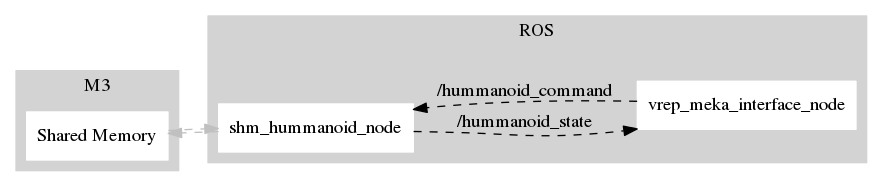
\includegraphics[width=1\linewidth]{figs/shm_arch}
    \caption{Arquitetura Controle C++}
    \label{fig:shm_arch}
\end{figure}

Todo o código relacionado ao controle do robô é disponibilizado pelo fabricante e compõe a biblioteca M3, implementada em Python e com interface em C++. Dentro do programa de interface com o ROS pela análise do código foi possível observar alguns pontos importantes dos controladores controladores de posição com e sem compensação da gravidade. Os valores de velocidade e torque informados para o controle são completamente ignorados. Além disto a taxa de envio da informação obtida pelo ROS para a memória compartilhada é de apenas $100Hz$ definidos \textit{hardcode}. Foi feito um teste para alterar este valor para $1KHz$ porém o robô ficou completamente instável. De movo que testes similares não foram repetidos para evitar danos ao robô.

Notadamente o valor de $100Hz$ é bem próximo das taxas de amostragem de $8 ms$ ($125 hz$) e $20 ms$ ($50 Hz$) utilizadas pelos controladores implementados em C++ obtidas para os melhores resultados em \cite{marcosps2016} obtidos por Marco Pereira. Sendo estes valores definidos pelo tempo mínimo necessário para efetuar todos os cálculos relacionados ao controladores cinemáticos implementados usando quatérnions duais.

\section{Estudo Controladores M3}

O sistema de controle M3 fornece diversos controladores e incorporados a plataforma. Para avaliar o desempenho dos controladores já existes foram feitos alguns experimentos, detalhados a seguir.

\subsection{Código de Demonstração}

São disponibilizados alguns códigos de exemplo em Python e C++, espalhados ao longo do código fonte da M3. Para estudo sobre controlar o robô a partir do código em Python foi tomado como referência o estudo dos códigos de demonstração e a documentação disponibilizada no site ReadTheDocs\footnote{\url{https://meka-docs.readthedocs.io/en/latest/}}. Neste processo foi adicionada mais uma pose no código de demonstração com o nome de referência \textit{Kojiref} com os valores usados para a posição inicial pelo Rafael Koji em \cite{koji2017}.

Para referência do uso dos controladores foi tomado como parâmetro inicial o código de demonstração sobre o controle de rigidez disponibilizado pelo fabricante, cuja interface gráfica é mostrada na figura \ref{fig:m3demo}. Na interface estão disponíveis algumas poses para mostrar o robô em posição estática, uma trajetória montada por uma sequência de poses e uma trajetória de um circulo elaborada a partir de splines. É possível ajustar a velocidade máxima e a rigidez do controlador de forma dinâmica, permitindo a avaliar o impacto na resposta do robô.

\begin{figure}[H]
    \centering
    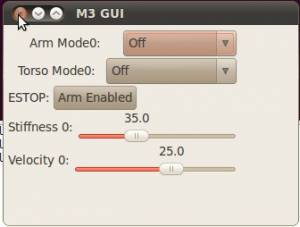
\includegraphics[width=0.5\linewidth]{tex/figs/mekademo.png}
    \caption{Interface Código de Demonstração \cite{mekaguide}}
    \label{fig:m3demo}
\end{figure}

A partir da execução do código de demonstração foi possível perceber que a posição das juntas varia conforme o valor de rigidez é ajustado. O valor da velocidade máxima e da rigidez variam de 0 a 1 internamente do código representando uma porcentagem do valor máximo possível. Ao que foi notado que mesmo com a rigidez no máximo o braço continua demonstrando um comportamento complacente. Com a rigidez em zero o controle é instável e o robô não consegue manter a posição e para valores abaixo de 0.2 o desempenho na execução de uma trajetória é visivelmente ruim.

% - A trajetória em circulo foi melhor ou pior que o trabalho do Marcos?

\subsection{API Python}

Como a maior parte do código da M3 está implementada em Python, para avaliar os controladores de junta de baixo nível foi utilizado a API para Python por ser a opção mais completa em termos de recursos. Sendo utilizada para todos os testes iniciais. No entanto, para registrar os valores do sensor foram registrados via \textit{rosbag} a partir das leitura do tópico $/hummanoid\_state$. Foi escolhido usar o programa rosbag em conjunto com o nó de ros $shm\_humanoid\_interface$ no lugar do registro direto em arquivo para facilitar a reproduzibilidade dos experimentos e análises feitas. Através interface da API em Python para a M3 estão estão disponíveis os seguintes controladores, ordenados do de mais alto nível para o de mais baixo nível:

\begin{itemize}
    \item Posição
    \item Velocidade
    \item Torque
    \item PWM
\end{itemize}

Os modos de controle de posição estão ainda disponíveis com e sem controle de compensação da gravidade a partir do modelo dinâmico inverso da M3 e obtido pelo algoritmo de dinâmica inversa de cadeia cinemática da biblioteca Orocos KDL\footnote{\url{http://www.orocos.org/KDL}}.

\subsubsection{Avaliação do Atraso de Comunicação}\label{subsec:deadtimepython}

A comunicação com o robô é feita através de uma memória compartilhada. Assim, o primeiro experimento foi levantar o tempo gasto pela instrução \textit{proxy.step()} que atualiza esta memória pegando as medidas dos sensores e informando os comandos para os controladores. Este teste foi feito através avaliando o intervalo de tempo entre cada chamada após sucessivas interações tendo como resultado o valor médio de 16ms entre cada chamada indicando que a frequência máxima possível para um controlador implementado com base na API é de $f = 1/16ms = 62.5Hz$. Isto, obviamente, desconsiderando qualquer tempo extra gasto com as operações realizadas pelo próprio controlador.

\subsubsection{Avaliação do Acumulo do Erro}

Para verificar o acumulo do erro após sucessivas interações foi feito o teste de fechar a malha com braço na posição de repouso. Isto é, controle deveria ler os dados atuais do sensores e passar diretamente para o robô na expectativa de que o robô ficasse parado. No entanto foi observado que o braço começou a subir lentamente, indicando valores cada vez maiores para os ângulos medidos e uma distância cada vez maior da posição de origem.

Por outro ao ser enviado a mesma posição de referência suscetivamente, o braço desloca até o ponto desejado e permanece parado, mostrando que o controle para um referência em degrau é estável. O que viabilizou os testes de identificação a partir do uso de uma entrada em Degrau.

\subsubsection{Acompanhamento de Referência}

No intuito de avaliar o comportamento dos controladores com um referência  com variação fixa da velocidade foram então feitos testes para uma entrada em rampa. Como se trata de um controle feito de maneira discreta, foram passados valores de ângulos em sequência incrementados por um valor contante e separados por um pequeno tempo de espera emulando uma entrada em rampa porém discretizada no tempo.

Para estudo da velocidade de resposta do controlador, o valor incrementado entre um ângulo e outro foi mantido enquanto o intervalo de tempo era ajustado. Neste experimento foi observado que para intervalos muito pequenos de tempo o robô não consegue acompanhar mantendo uma velocidade constante. Em tais casos a velocidade é mantida aproximadamente constante e com o acúmulo do erro ocorre saltos periódicos para compensar o atraso em relação a referência. Este fato decorre da interação entre o controlador de posição das juntas e o controlador de torque. O erro acumulado é corrigido com a passagem de um torque mais alto produzindo um salto na posição, seguido de uma leve oscilação para compensar o efeito da inercia.

% Repete testes ?

\subsubsection{Resposta ao Degrau}

Feito uma avaliação preliminar para o experimento de identificação da planta foi aplicado um degrau para cada uma das juntas individualmente com registro dos dados. Este teste foi definido a partir dos seguintes passos:

\begin{enumerate}
    \item Começa com a junta na posição $0$ graus
    \item Envia o comando para ir para posição $45$ graus
    \item Mantém a referência da posição em $45$ graus por $2s$
    \item Envia o comando para ir para posição $0$ graus
    \item Mantém a referência da posição em $0$ graus por $2s$
\end{enumerate}

Para a API em Python estes passos foram executados 3 vezes para cada uma das juntas. Um experimento semelhante foi efetuado a partir de um programa em C++ baseado no código elaborado em trabalhos anteriores. Para ambos casos a saída dos sensores foi registrada a partir do ROS a partir do programa \textit{rosbag} e somente para os testes feitos em C++ foram também registradas os mensagens de controle. Uma vez que os comandos passados via API são enviados diretamente para o serializador de mensagens sem passar pelo ROS e portanto foram utilizados apenas para uma avaliação preliminar do comportamento dos controladores de junta. Mais detalhes do experimento em C++ na seção \ref{subsec:stepcpp}. 

% Qual foi a diferença dos dois para os mesmo parâmetros?
% Por que não foram avaliados outros ângulos?

\subsubsection{Controle de Posição sem Compensação da Gravidade}

O controle de posição sem o uso de compensação da gravidade foi avaliado em estudo e não foi possível atingir a posição desejada de 45 graus partido do zero em nenhuma das juntas. Na maioria dos caso o braço movia apenas 10 graus. O que explicita o fato do impacto de toda a estratégia de compensação da gravidade ser feita por software. A precisão do controle, depende da qualidade do modelo dinâmico e da estratégia utilizada. Esta solução que o sistema de controle possa ser sempre atualizado, uma vez que não está embutido no projeto de hardware, no entanto fica preso a qualidade do modelo.

\subsubsection{Controle de Velocidade}

Na hipótese de utilizar um controle de baixa nível de velocidade ao invés de posição, foi feito apenas um ensaio utilizando o controle de velocidade disponível na API em Python. No entanto ao ser definido velocidade zero a braço robótico ficou completamente rígido e passou a ignorar comandos para outros valores de referência de velocidade. O que demonstrou um esforço grande sendo feito pelo controle de torque e pelos motores. Somente quando foi alterado o modo de controle para posição que o braço voltou a mover normalmente. Para evitar qualquer dano a plataforma, não foram feitos outros testes neste modo de operação. Em \cite{mekartfd} este modo de controle foi classificado como instável, recomendando evitar o uso pois o sinal da velocidade possui muito ruído pois o sinal é estimado no computador através de diferenças finitas a partir da leitura da posição.

% Teria como controlar a velocidade diretamente ?

%\subsubsection{Controle de Torque}

%O controle de torque está disponível em dois modos: com e sem compensação da gravidade. Na estratégia sem compensação da gravidade, o valor de referência de torque é passado diretamente a controlador das juntas.

% Por que não foi avaliado o controle de torque?

\section{Estudo Controladores Cinemáticos}

Em C++ não estão disponíveis todos os modos de operação para o uso a partir do ROS, embora ao final a mensagem seja serializada e passada para os mesmos programas. No nó $shm\_hummanoid$ está implementado somente o controle por posição com e sem compensação da gravidade. Em decorrência disto, foi analisado somente o controlador de posição com compensação da gravidade por ter sido o utilizado em trabalhos anteriores. Os tempos foram obtidos a partir do $ros::time$ e registrado nas mensagens como \textit{timestamp}. Foi necessário alterar o código do $vrep\_meka\_interface$ para incluir o \textit{timestamp} na mensagem para permitir a análise dos dados registrados via \textit{rosbag}. Em razão disto, alguns dos experimentos anteriores não foram incluídos no estudo do tempo de resposta por conta de inexistir um referencial de tempo comum para as mensagens do tópico $/hummanoid\_state$ e $/hummanoid\_command$.

\subsection{Controle de Posição de Juntas}\label{subsec:stepcpp}

Para avaliar a resposta do controlador em C++ foi aplicado um degrau para cada uma das juntas individualmente com registro dos dados. Este teste foi definido a partir dos seguintes passos:

\begin{enumerate}
    \item Começa com a junta na posição $0$ rad
    \item Envia o comando para ir para posição $1$ rad
    \item Mantém a referência da posição em $1$ rad por $4s$
    \item Envia o comando para ir para posição $0$ rad
    \item Mantém a referência da posição em $1$ rad por $4s$
\end{enumerate}

Estes passos foram repetidos, ajustando-se os os parâmetros de rigidez e velocidade máxima do controlador. A velocidade máxima de cada junta pode ser ajusta para um valor entre $0$ e $1$, de igual forma a rigidez do braço gerada pelo controlador também pode ser ajustada entre $0$ e $1$. Valores maiores que 1 foram testados porém não houve mudança significativa em relação a comportamento com valor $1$. Muito embora em trabalhos anteriores na plataforma fosse usado $rigidez = 5$. Vale reforçar que estes são parâmetros usados pelos controladores no PC ( posição e compensação da gravidade ) de forma que não é possível obter diretamente os parâmetros de rigidez e velocidade máxima pela resposta do estado atual fornecida por \textit{/hummanoid\_state} pois a complacência do controlador é ajusta por software.

Já no experimento feito de referência mostrado na \ref{fig:jointIdentification_exp2v100v50}, pode-se notar que existe um atraso de cerca de $20ms$ entre o comando e o recebimento do sinal de resposta do atuador no tópico. Também percebe-se um erro grande em regime permanente das juntas do pulso ($5$ e $6$). Percebe-se uma longa rampa indicando aonde o controle da posição passou a atuar como um controle tudo ou nada passando a velocidade máxima possível. Curiosamente, embora sejam motores distintos em cada uma das juntas com diferentes limites de velocidade a resposta dpelo gráfico percebe-se uma velocidade próxima de $V = 1.5 rad/s$. O que mostra que os controladores de posição estão ajustados para operarem na faixa linear comum a todos os motores, que é abaixo da velocidade máxima do junta mais lenta $J4$ de $V_4 = 2.0 rad/s$, conforme registrado na tabela \ref{tab:a2armActuationDoc}. De forma que um controlador mais sofisticado pode ser desenvolvido de modo a permitir explorar melhor a capacidade das juntas mais rápidas.

\begin{figure}[H]
    \centering
    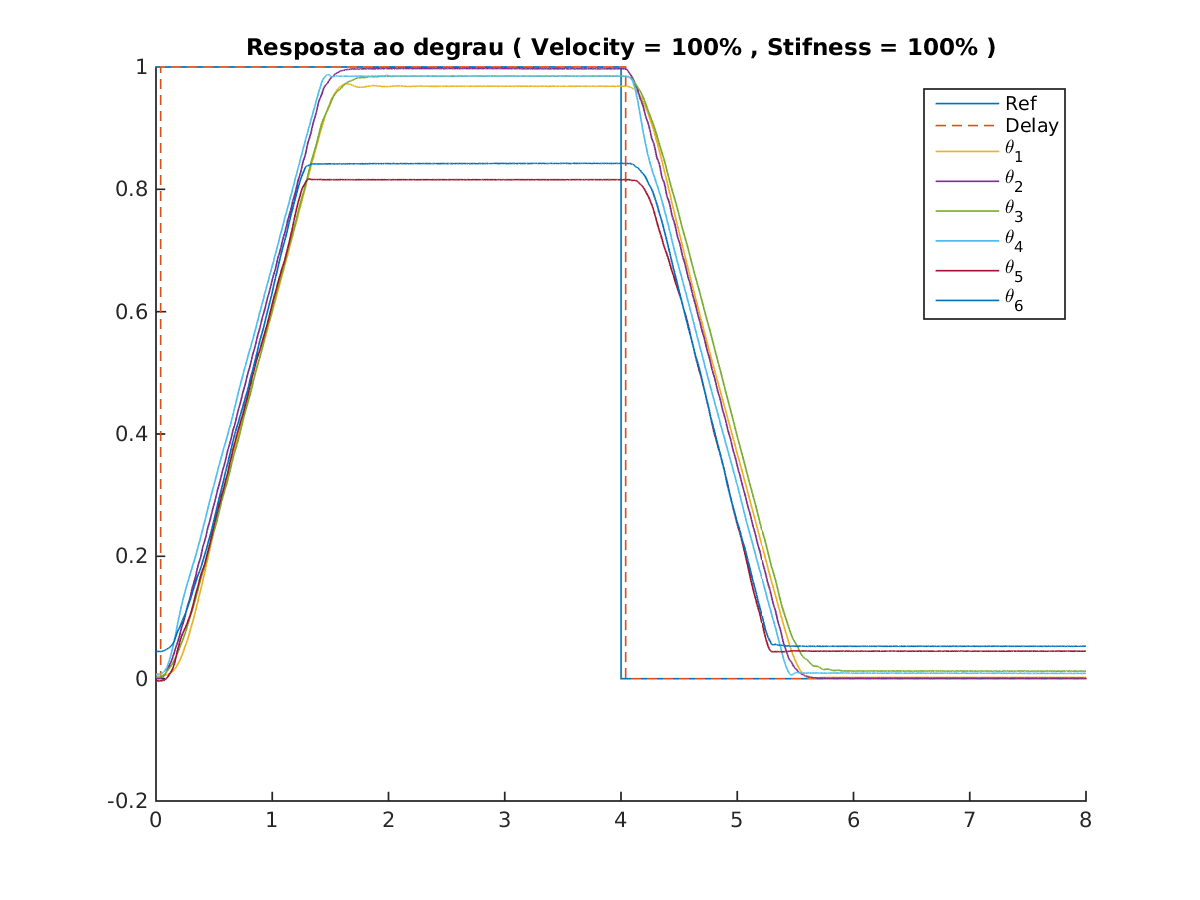
\includegraphics[width=0.8\linewidth]{tex/figs/jointIdentification_exp1v100v100.png}
    \caption{Resposta a um degrau de entrada com Velocidade = 1 e Rigidez = 1}
    \label{fig:jointIdentification_exp1v100v100}
\end{figure}

Pela figura \ref{fig:jointIdentification_exp2v100v50} observa-se que a variação da rigidez do controlador implica em um erro maior em regime permanente nas juntas. O controlador converge em um tempo próximo mas notadamente aumenta o erro das juntas do pulso. Este fato também é percebido no código de demonstração no ajuste da rigidez. Tendo sido notado que ao mudar o valor do parâmetro de rigidez na interface com o robô parado sem alterar a posição de referência desejada o pulso desloca significativamente de posição.

\begin{figure}[H]
    \centering
    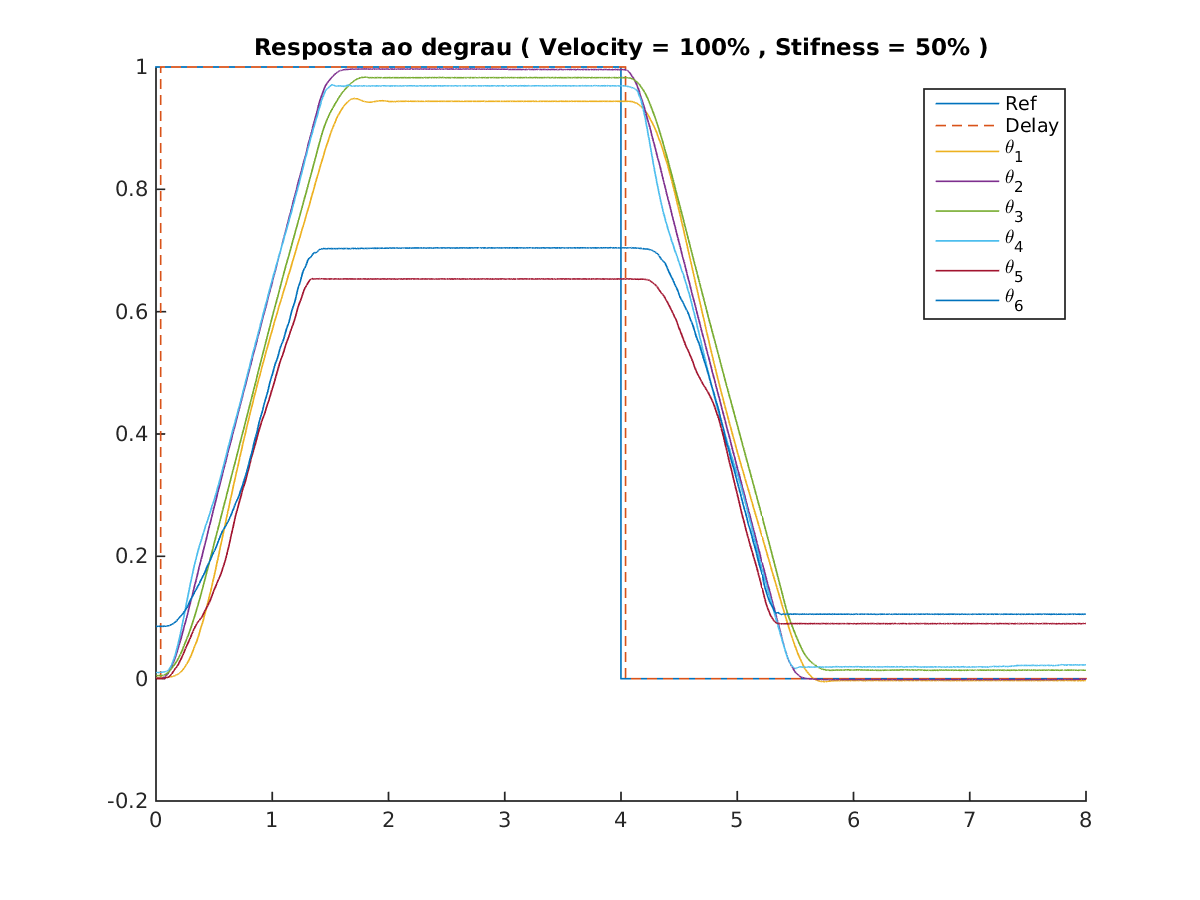
\includegraphics[width=0.8\linewidth]{tex/figs/jointIdentification_exp2v100v50.png}
    \caption{Resposta a um degrau de entrada com Velocidade = 1 e Rigidez = 0.5}
    \label{fig:jointIdentification_exp2v100v50}
\end{figure}

Como esperado, no terceiro experimento ao se alterar a velocidade para $70\%$ o tempo necessário para cada uma das juntas atingir a posição aumentou, tendo em vista a fase em que o controlador utiliza a velocidade máxima permitida, o erro em regime permanente para cada um permanece com pouca alteração. No entanto é percebido que a inclinação da curva durante as fase de controle entre o tempo $t=1s$ e $2s$ com a velocidade máxima muda de forma diferente para cada uma duas juntas. Estes dados encontram-se na figura \ref{fig:jointIdentification_exp3v70v100}.

No 3 experimentos o atraso obtido foi próximo de $20ms$. Este valor é próximo dos valores de intervalo de tempo obtidos para os melhores resultados dos controladores implementados em \cite{marcosps2016} e também próximo do valor obtido na seção \ref{subsec:deadtimepython}. O que reforça a tese boa parte do atraso ocorre devido a camadas abaixo do nó de ROS. Notadamente, quando o controlador opera com frequências maiores, o impacto do atraso da comunicação passa a ser mais significativo levando a instabilidade caso este não seja considerado no dinâmica implementada como obtido experimentalmente por Marcos. Para uma análise mais completa da resposta das juntas é sugerido o uso de variações menores de ângulo como forma de evitar a não lineridade devido a saturação dos motores.

\begin{figure}[H]
    \centering
    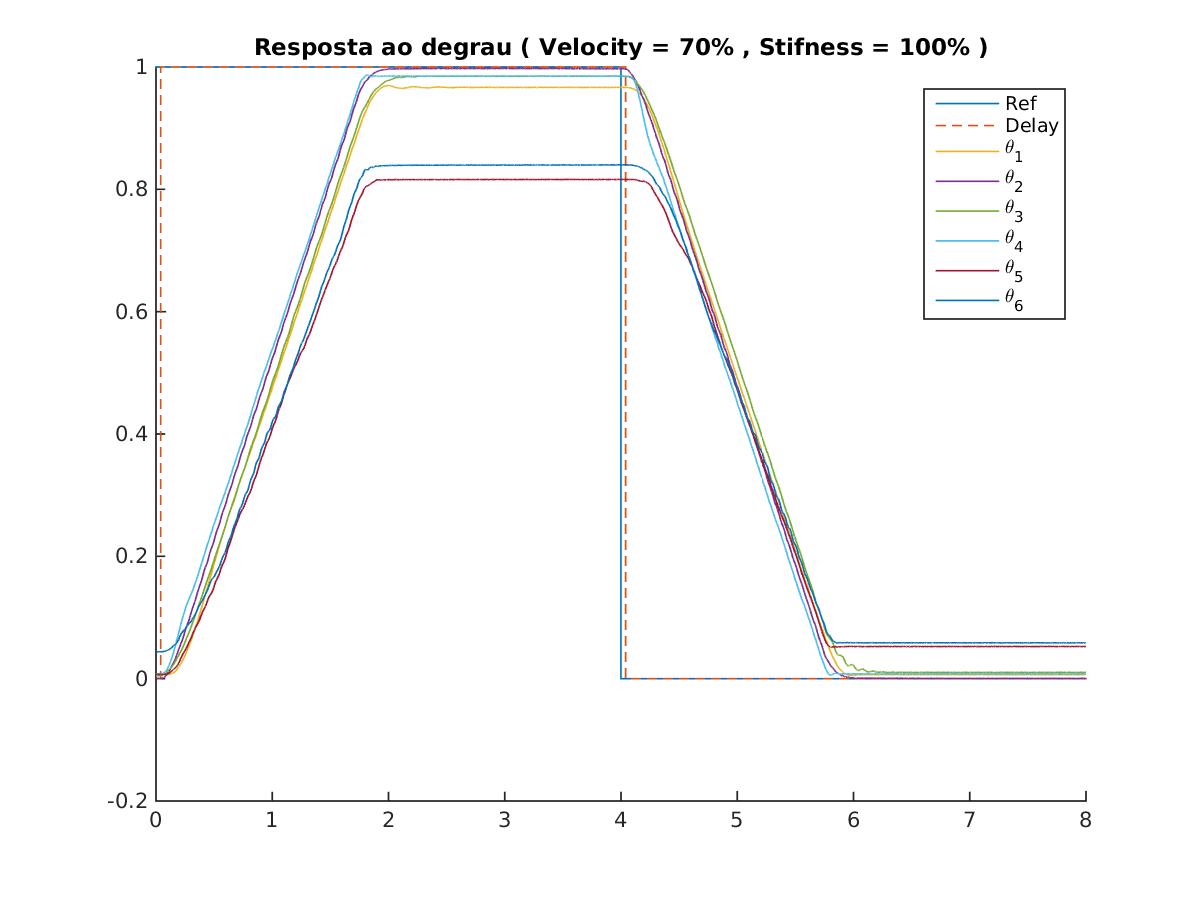
\includegraphics[width=0.8\linewidth]{tex/figs/jointIdentification_exp3v70v100.png}
    \caption{Resposta a um degrau de entrada com Velocidade = 0.7 e Rigidez = 1}
    \label{fig:jointIdentification_exp3v70v100}
\end{figure}

% Comentar sobre o varição do intervalo de tempo medido da entre os comandos enviados para a \hummanoid_command

Tomando-se o diferença entre o valor passado de referência e o valor alcançado tempo foram obtidos os erro em regime permanente, registrados na tabela \ref{tab:jointIdentification_errortable}.

\begin{table}[H]
    \centering
    \caption{Error Percentual para diferentes valores de velocidade ($V$) e rigidez ($S$)}
    $$\begin{array}{cc|ccccccc}
         \hline
         V & S & \theta_0 & \theta_1 & \theta_2 & \theta_3 & \theta_4 & \theta_5 & \theta_6\\
         \hline
         -Inf & 0.031544 & 0.0025193 & 0.014824 & 0.014865 & 0.18436 & 0.15769\\
-Inf & 0.056071 & 0.0036188 & 0.017413 & 0.031003 & 0.34662 & 0.29566\\
-Inf & 0.033305 & 0.0026167 & 0.015199 & 0.014783 & 0.18398 & 0.16037\\
-Inf & 0.056453 & 0.0035564 & 0.017352 & 0.03028 & 0.32879 & 0.28538\\

         \hline
    \end{array}$$
    \label{tab:jointIdentification_errortable}
\end{table}

\begin{table}[H]
    \centering
    \caption{Percentual Overshot para diferentes valores de velocidade ($V$) e rigidez ($S$)}
    $$\begin{array}{cc|ccccccc}
         \hline
         V & S & \theta_0 & \theta_1 & \theta_2 & \theta_3 & \theta_4 & \theta_5 & \theta_6\\
         \hline
         0 & 1.0041 & 1.0001 & 1.0002 & 1.0025 & 1.0016 & 0\\
0 & 1.0049 & 1.0004 & 1.0008 & 1.0019 & 1.0007 & 0\\
0 & 1.003 & 1.0002 & 1.0004 & 1.0016 & 0 & 0\\
0 & 1.005 & 1.0004 & 1.0009 & 1.0026 & 0 & 0\\

         \hline
    \end{array}$$
    \label{tab:jointIdentification_overshottable}
\end{table}

\begin{table}[H]
    \centering
    \caption{Valor em regime permanente para diferentes valores de velocidade ($V$) e rigidez ($S$)}
    $$\begin{array}{cc|ccccccc}
         \hline
         V & S & \theta_0 & \theta_1 & \theta_2 & \theta_3 & \theta_4 & \theta_5 & \theta_6\\
         \hline
         1.00 & 1.00 & 0.001841 & 0.96846 & 0.99748 & 0.98518 & 0.98513 & 0.81564 & 0.84231\\
1.00 & 0.50 & 0.003698 & 0.94393 & 0.99638 & 0.98259 & 0.969 & 0.65338 & 0.70434\\
0.70 & 1.00 & 0.0020654 & 0.9667 & 0.99738 & 0.9848 & 0.98522 & 0.81602 & 0.83963\\
1.00 & 0.50 & 0.0047216 & 0.94355 & 0.99644 & 0.98265 & 0.96972 & 0.67121 & 0.71462\\

         \hline
    \end{array}$$
    \label{tab:jointIdentification_steadstatetable}
\end{table}

% Acrescentar Tempo de Resposta 

\subsection{Avaliação na execução de Trajetória em linha reta}

% Obter dt em /hummanoid_state e /hummanoid_command para cada um dos casos
% Experimento MoveUP

Os controladores de posição do efetuador foram avaliado a partir da estratégia de discretização dos pontos e frequência de amostragem. Para tal foi reduzido o número de ponto e trajetória foi simplificada para apenas um deslocamento em linha reta de 10cm na vertical. Para primeira análise foi utilizado os controladores implementados anteriormente e foram feitos os seguintes testes:

\begin{enumerate}
    \item Trajetória dividida em $100$ pontos, intervalo de $8 ms$
    \item Trajetória dividida em $100$ pontos, intervalo de $100 ms$
\end{enumerate}

Foi observado que o robô leva um tempo até começar a mexer e um tempo até o controle estabilizar. De modo que está sempre atrasado em relação a referência. Para o período $8 ms$ foram necessárias $25$ interações até o robô começar a se mover, com o período de $100 ms$ o robô começo a se mover já na segunda interação sugerindo um atraso de $200 ms$ entre o tempo que o comando é passado via ROS e o tempo que o robô executa o comando.

% Gráficos ?

Assim foram feitos novos experimentos para as seguintes variações:

\begin{enumerate}
    \item Trajetória dividida em $100$ pontos, $velocidade em 100\%$, intervalo de $2 ms$
    \item Trajetória dividida em $100$ pontos, $velocidade em 100\%$, intervalo de $10 ms$
\end{enumerate}

No primeiro experimento, figura \ref{fig:moveUp1}, o robô executou a trajetória sem problemas movendo para cima com velocidade constante.

\begin{figure}[H]
    \centering
    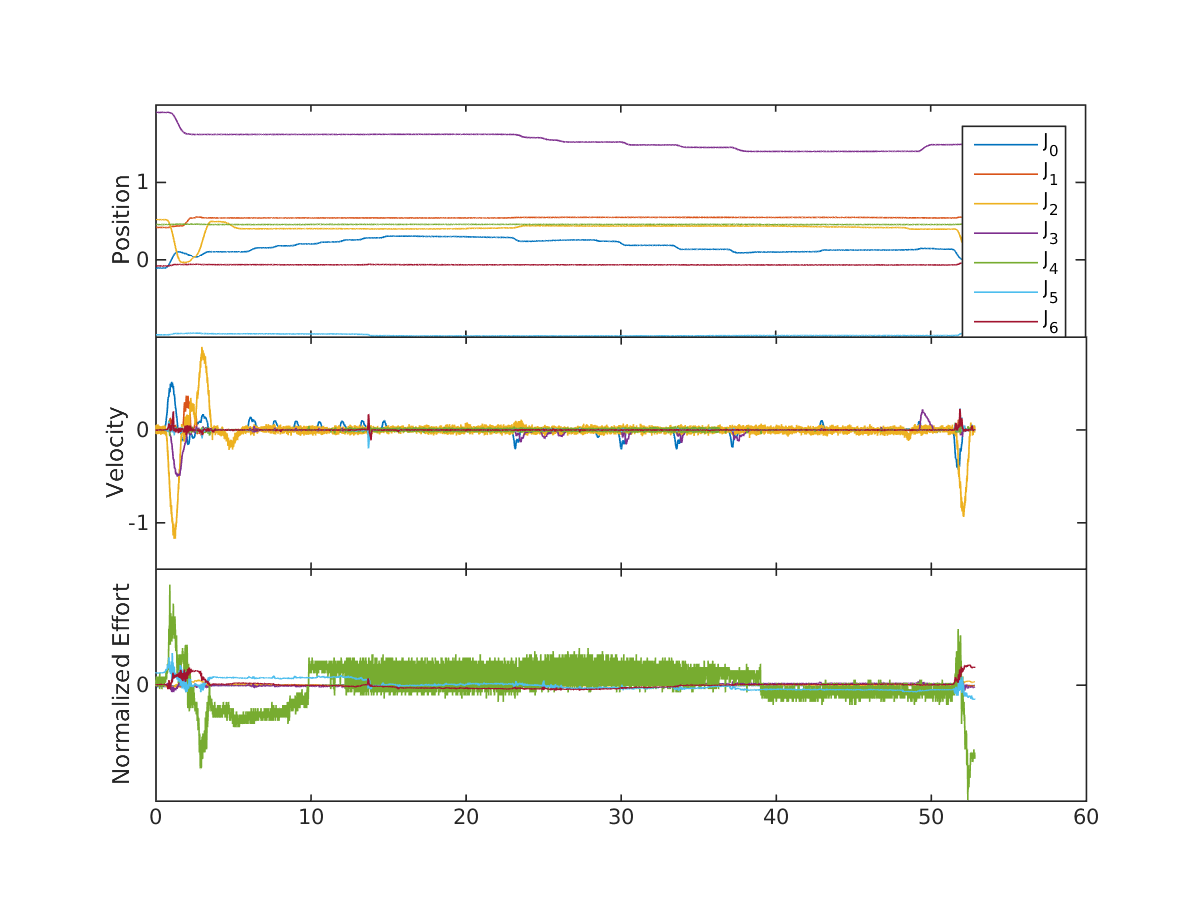
\includegraphics[width=0.6\linewidth,trim={2cm 1cm 2cm 2cm}]{tex/figs/moveUp1stateEvalv70s10.png}
    \caption{Experimento Trajetória na Vertical $dt=10ms$ }
    \label{fig:moveUp1}
\end{figure}

Já quando o intervalo de tempo entre os pontos é muito abaixo de $20ms$ é percebido saltos periódicos com intervalo aproximado de $5s$ devido ao acumulo do erro nas juntas. Nota-se que as juntas movem em velocidade constante por um tempo e em seguida rola o salto. Dá para notar que as juntas $J5$ e $J6$ são as que possuem a maior variação no esforço ao longo da trajetória.

\vspace{1cm}

\begin{figure}[H]
    \centering
    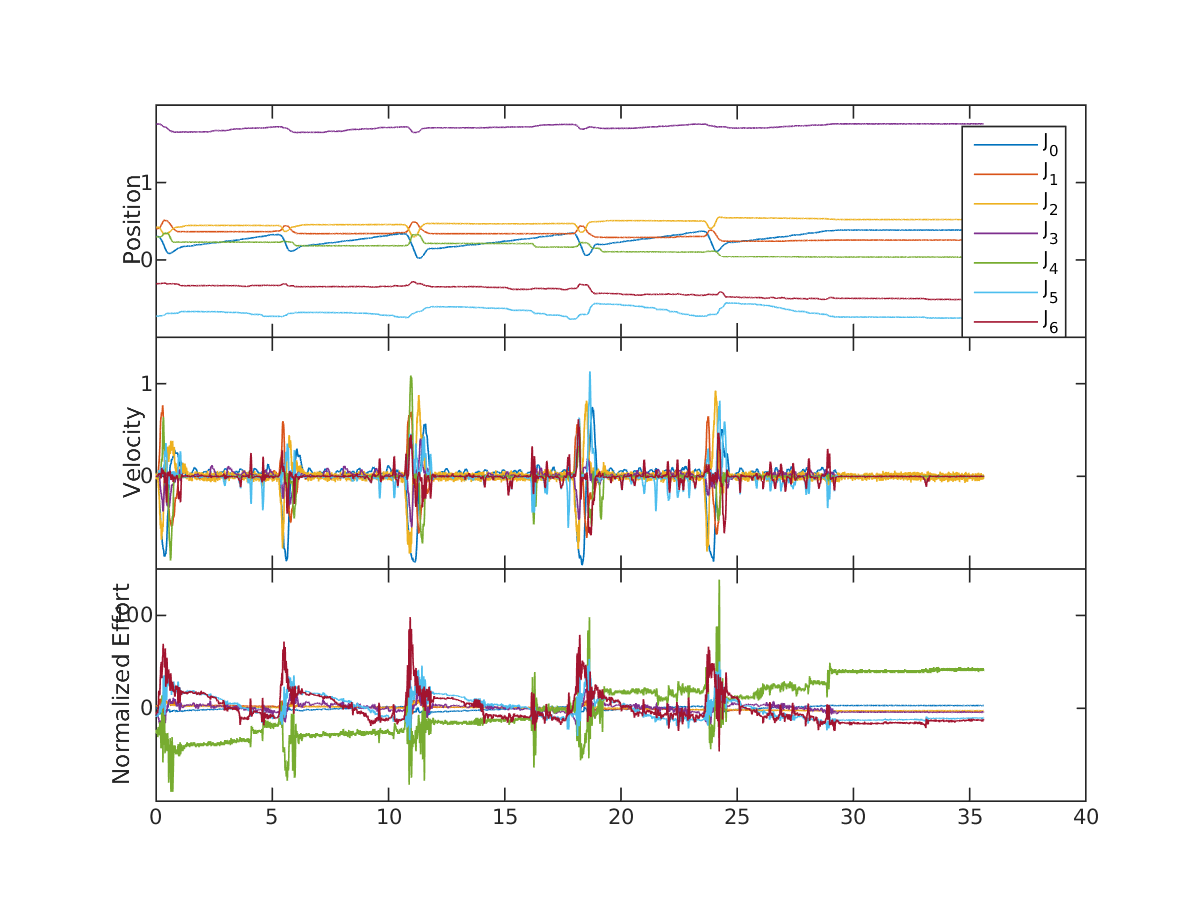
\includegraphics[width=0.6\linewidth,trim={2cm 1cm 2cm 2cm}]{tex/figs/moveUp3stateEvalv70s50.png}
    \caption{Experimento Trajetória na Vertical $dt=2ms$ }
    \label{fig:moveUp3}
\end{figure}

% Saltos a cada 300 ms

\section{Estudo de saturação da velocidade dos atuadores}

Em extensão ao estudo feito na seção \ref{subsec:stepcpp}, foi analisado a resposta da velocidade fornecida pelo tópico ao longo da trajetória. Pelas figuras \ref{fig:jointIdentification_exp1v100v100}, \ref{fig:jointIdentification_exp2v100v50} e \ref{fig:jointIdentification_exp3v70v100} foi notado notado que a velocidade é aproximadamente constante ao longo dos momentos de maior deslocamento e com valores próximos de $v_{max} = 0.5 rad/s$ para todas as juntas. Para avaliar o comportamento ao longo do tempo foi comparado a resposta fornecida no tópico do ROS $/hummanoid\_state$ para os valores de \textit{position}, \textit{velocity} e \textit{effort}, respectivamente posição, velocidade e torque nas juntas, conforme mostrado nas figuras \ref{fig:jointIdentificationFullSpeed_stiff90p} e \ref{fig:jointIdentificationSpeed10p_stiff90p2}.

\vspace{1cm}
\begin{figure}[H]
    \centering
    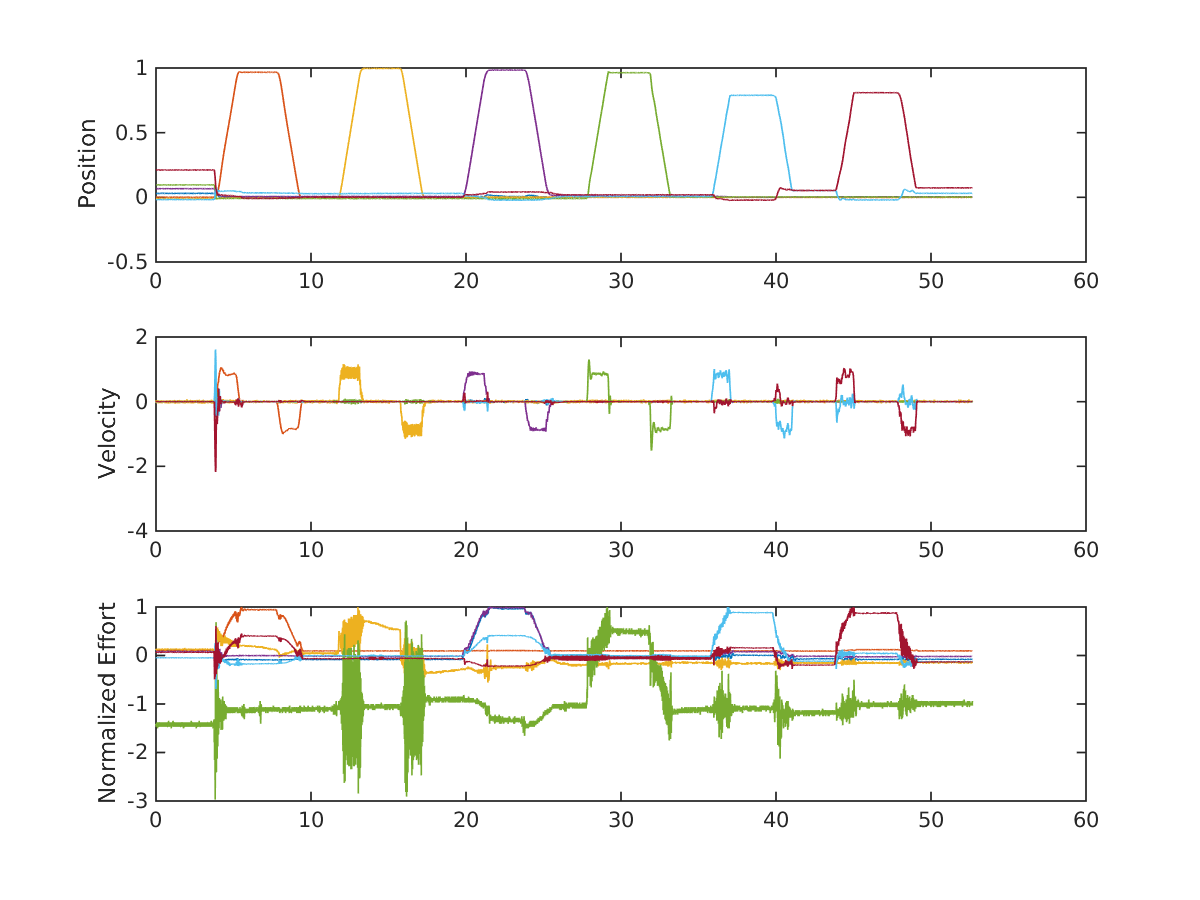
\includegraphics[width = \linewidth]{tex/figs/jointIdentificationFullSpeed_stiff90p.png}
    \caption{Resposta Controladores Juntas - Velocidade Máxima e 90\% de rigidez}
    \label{fig:jointIdentificationFullSpeed_stiff90p}
\end{figure}

A medida do torque varia bastante de junta para junta, uma vez que o esforço necessário para mover o braço inteiro é bem menor que para mover cada uma das partes. Em razão disto foi feito um ajuste nos valores de $effort$ a dividindo os valores ao longo da trajetória pelo valor máximo observado em cada junta para permitir avaliar o formato da resposta do torque de forma igual para todas as juntas.

% Resposta do Sensor
Obviamente a velocidade é apenas uma estimativa da velocidade real a partir do valor de posição que chega no computador. Pois, como mostrado na tabela \ref{tab:a2armSensorDoc} não existe um sensor de velocidade embarcado em cada uma das juntas, apenas sensores de posição. Este valor é notadamente ruidoso pois devido ao atraso de comunicação e detecção, a medida dos valores de posição também sofre de não linearidades, apresentando apresentando momentos em que esta não varia.

Ao que é percebido a origem do ruído na medida da velocidade: em momentos que o informação da posição é consultada na memória compartilhada antes da informação ser atualizada gera uma velocidade nula, uma vez que não houve variação do dado. Consultando os códigos foi notado que o valor da medida da estimativa é filtrado por um filtro passa baixa de Butterworth de 3 ordem com frequência de corte em $80 Hz$ para cada uma das juntas. O que atenua um pouco do efeito da estimativa da derivada porém ainda assim a confiabilidade da medida é bem menor que a de posição e torque.

% Valores Extraídos de robot_config/ma_26/m3actuator_ma26_j4
% Montar tabela com todos os atuadores
% angle_df:
%     theta_df:
%       cutoff_freq: 80
%       order: 3
%       type: butterworth
%     thetadot_df:
%       cutoff_freq: 20
%       order: 3
%       type: diff_butterworth
%     thetadotdot_df:
%       cutoff_freq: 20
%       order: 3
%       type: diff_butterworth
%     type: df_chain

Dado que a velocidade máxima da junta mais rápida é de $4.6 rad/s$ a variação máxima esperada é de $f_0 = 1/(2pi/4.6 rad/s) = 0.732 Hz$, A frequência de corte $f_{filt} = 80Hz$ representa em torno $10 f_0$. Como este tipo de filtro não leva em consideração o modelo físico do processo, apenas a resposta em frequência, outros tipos de filtro podem ser implementados, visando melhorar a qualidade da estimativa.

Para avaliar a situação em que a velocidade máxima é abaixo do necessário para permitir o controlador convergir foi refeito o experimento com o mesmo valor de rigidez e $10\%$ da velocidade máxima (Figura \ref{fig:jointIdentificationSpeed10p_stiff90p2}). Nesta situação nota-se uma variação maior para as velocidades apresentadas para as juntas de menor velocidade $J4$, $J5$ e $J6$. A junta do cotovelo $J4$ em particular foi a que apresentou o maior erro. Também não foi possível atingir o ponto de referência no intervalo dado. Em lugar temos uma resposta em formato triangular indicando a saturação da velocidade na subida e na decida. O que também é possível para notar no gráfico da velocidade.

\begin{figure}[H]
    \centering
    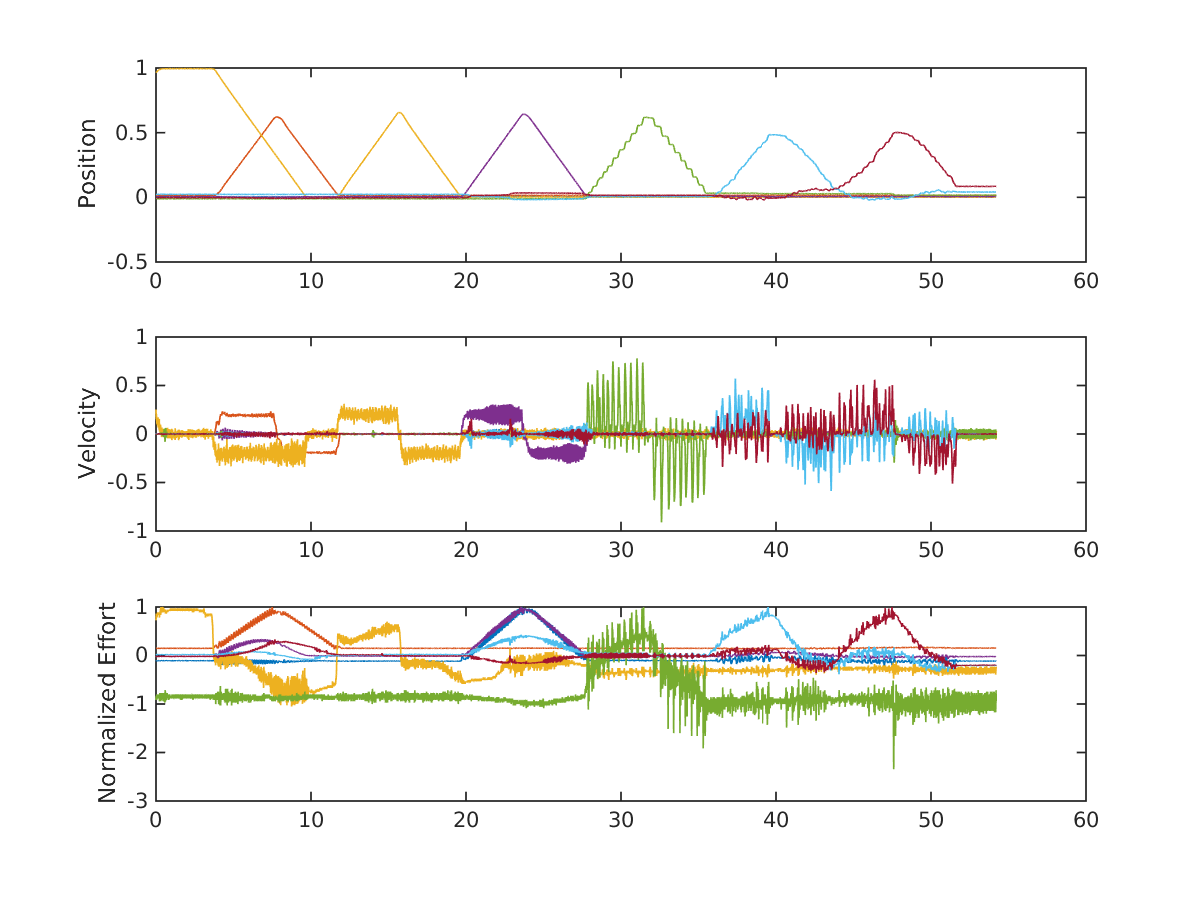
\includegraphics[width = \linewidth]{tex/figs/jointIdentificationSpeed10p_stiff90p2.png}
    \caption{Resposta Controladores Juntas - Velocidade em 10\%e rigidez em 90\%}
    \label{fig:jointIdentificationSpeed10p_stiff90p2}
\end{figure}

%\section{Estudo sobre não linearidades}

% Acrescentar simulação no simulink pControlSaturation
% - Comparativo da resposta para o mesmo ganho em um sistema de primeira ordem ( com delay e saturação )
% - Verificar necessidade de mudar a ordem e puxar a seção para antes

Uma vez que os modelos usados para o controle são lineares, a existência de comportamentos não lineares como saturação representam perturbações e podem gerar erros ou até instabilidade no controle caso não consideradas. Em razão disto uma atenção especial foi dada a este aspecto visando identificar a contribuição na perca de desempenho. A grande dificuldade é que ocorrem ao longo de todo o processo, principalmente devido a discretização, gerando um acumulo do efeito com o aumento da quantidade de camadas em cascata.

\subsection{Saturação do Atuador na Trajetória}

O efeito de saturação do atuador ocorre quando é solicitado uma ação de torque ou velocidade acima do que o atuador permite. Em diversos sistemas isto é limitado através de algum dispositivo de proteção evitando danificar o atuador. Do lado do controle, este é percebido como uma resposta mais lenta que o esperado para aquele determinado ganho em simulação podendo levar a instabilidade no controle do sistema real devido ao acumulo do erro no integrador.

Como o controle da posição é feito em colaboração pela ação de cada uma das juntas, este problema é mascarado na métrica do erro de posição. A contribuição de cada junta em manipulador não cartesiano muda de acordo com a posição, o atraso devido a saturação pode fazer com que o robô tenha um erro maior para determinadas posições no decorrer da trajetória que outras. Outro efeito é a saturação de um motor levar a um uso maior dos outro motores na tentativa de compensar o erro acumulado. Como são utilizados diferentes motores para cada uma das juntas, conferindo limitações especificas na atuação, em particular na velocidades máximas que cada junta pode atingir. Por conta disto, é percebido um maior uso das juntas com velocidade máxima maior para compensar o erro acumulado pela juntas com velocidade máxima menor, quando o controle começa solicitar uma velocidade maior que a permitida pelos outros motores. Em particular no Meka, este fenômeno leva a um uso maior das juntas do ombro para corrigir orientação ao acumulado pela saturação das juntas do pulso.

Em um manipulador robótico composto por juntas rotacionais, a tarefa de deslocamento no espaço é distribuída entre todas as juntas ao longo de praticamente toda a região do espaço de trabalho. O deslocamento de cada junta produz um arco que inevitavelmente gera movimentação em pelo menos duas direções no espaço e uma rotação. Desta forma o tarefa de atingir uma posição e orientação no espaço é distribuída por várias juntas, permitindo um esforço menor em um determinado atuador. No entanto, em particular para um braço antropomórfico a orientação é resolvida de forma conjunta pelo pulso e pelo ombro gerando um amplo espaço nulo a permitindo para uma mesma posição do pulso, diversas posições para o cotovelo.

Tais relações geométricas indicam que a tarefa de manter uma orientação possui uma relação com o movimento necessário pelas juntas notadamente diferente da tarefa de manter uma posição. De forma a permitir separar a complacência da posição ou da orientação conforme necessário para a tarefa. Ao se utilizar a representação cinemática por Quatérnions Duais tanto a referência da posição como a da orientação estão acopladas. Um bom controlador por outro lado necessita de uma rápida resposta a uma perturbação, gerando uma rigidez maior ao invés de uma complacência. Como para os experimentos em questão a orientação de referência era mantida como a orientação inicial do robô, parte do esforço de controle era direcionado em manter a orientação. O que gerava uma pertubação na posição. Este problema em composição com diferença de velocidade dos atuadores do pulso e da ombro fazia com que uma perturbação na orientação percebida no pulso provoca-se uma movimentação juntas do ombro e por consequência uma movimentação da posição do cotovelo. O que gerava uma aproximação do cotovelo para a base provocando em cascata uma maior chance colisão do braço com o tronco e uma dificuldade em manter a estabilidade as referências do controle através da cinemática diferencial. Pois o robô se aproximava do limite da junta e de regiões com bloqueio de movimento.

As consequências deste fenômeno foram atenuadas pelos primeiro trabalhos com o acréscimo de uma espuma de proteção no tronco do robô, minimizando o risco de dano. Em \cite{marcosps2016} foi resolvida pelo Marcos Pereira pela escolha de posições iniciais com o cotovelo distante do tronco e operando em uma região limitada por um plano paralelo a frente do robô. Em \cite{koji2017}, Rafael Koji, apresenta como solução a separação do acoplamento do controle das 2 juntas do pulso ($j5$ e $j6$) com a redução do modelo cinemático do manipulador para 5 juntas apenas. O que permitindo o controle de posição em malha fechada com 5 graus de liberdade e a orientação em malha aberta pelas juntas do pulso, reduzindo as instabilidades. Em um experimento disponível no YouTube \footnote{https://sites.utexas.edu/hcrl/2010/11/09/experiments-on-prioritized-compliant-control/} Luís Sentis demonstra a utilização de campos potenciais como forma de manter a postura do robô e evitar a colisão enquanto permite a priorização do controle complacente em uma das 3 direções $X$, $Y$ e $Z$ a partir da arquitetura implementada em \cite{sentis2007synthesis} no Meka.

% aqui entra o kung-fu 

% Fenômeno Harakiri: O cotovelo do meka vai se aproximando do tronco com o passar do tempo, o robô move bruscamente com pertubações na orientação a partir da posição de referência usada nos trabalhos do Koji e do Marcos

% Montar experimentos Harakiri 2DOF, Harakiri Meka em simulação no Matlab, Harakiri Meka real
% Estudo do erro por junta ao invés de por posição -> Pontuar necessidade introduzir novas métricas

%\subsection{Atraso da Comunicação}

%Dado a existência de várias camadas entre o controle cinemático e o atuador de fato, existe um atraso na comunicação que influência na dinâmica do sistema. O controlador cinemático interagem com o ROS que por sua vez interage com uma memória compartilhada que é atualizada com um frequência de $1 KHz$. Para avalia o atraso foi feito a medida a partir do ensaio em degrau, entre o tempo de envio do comando de controle no tópico $/humanoid_control$ e o primeiro instante em que a posição da junta atinge um valor diferente de zero na leitura do valor correspondente no tópico $/humanoid_state$. Uma vez que existe um pouco de ruído na leitura da posição, foi considerado a valor de referência $\Delta\theta_0 = 0.1 rad = 5^\circ$.

% Resultados

%\subsection{Controle Virtual de Rigidez}

% Comparar com primeiras implementações de SEA

%Com base no controle do torque e o uso de sensores de posição pode se emular o comportamento de uma mola com rigidez variável através de um controlador. Esta estratégia é denominada mola virtual e permite conferir o controle de força com precisão sem a necessidade de ajustar fisicamente algum elemento elástico.

% Diagrama SEA Virtual

\section{Estudo Controladores Cinemáticos}

\subsection{Análise individual dos Controladores de Junta}

Para avaliar a variação da resposta dos controladores cinemáticos implementado primeiramente foi tomado como referência os resultados de trabalhos passados. No qual foi refeito o experimento da trajetória de um quadrado com todos os controladores ajustados para os melhores parâmetros obtidos em \cite{marcosps2016}, enquanto os parâmetros dos controladores de baixo nível foram mantidos. Neste experimento (Figura \ref{fig:squareStiffMarcos}) foi acrescentado a resposta da velocidade e do torque obtidos a partir do tópico $/humanoid\_state$.

\begin{figure}[H]
    \centering
    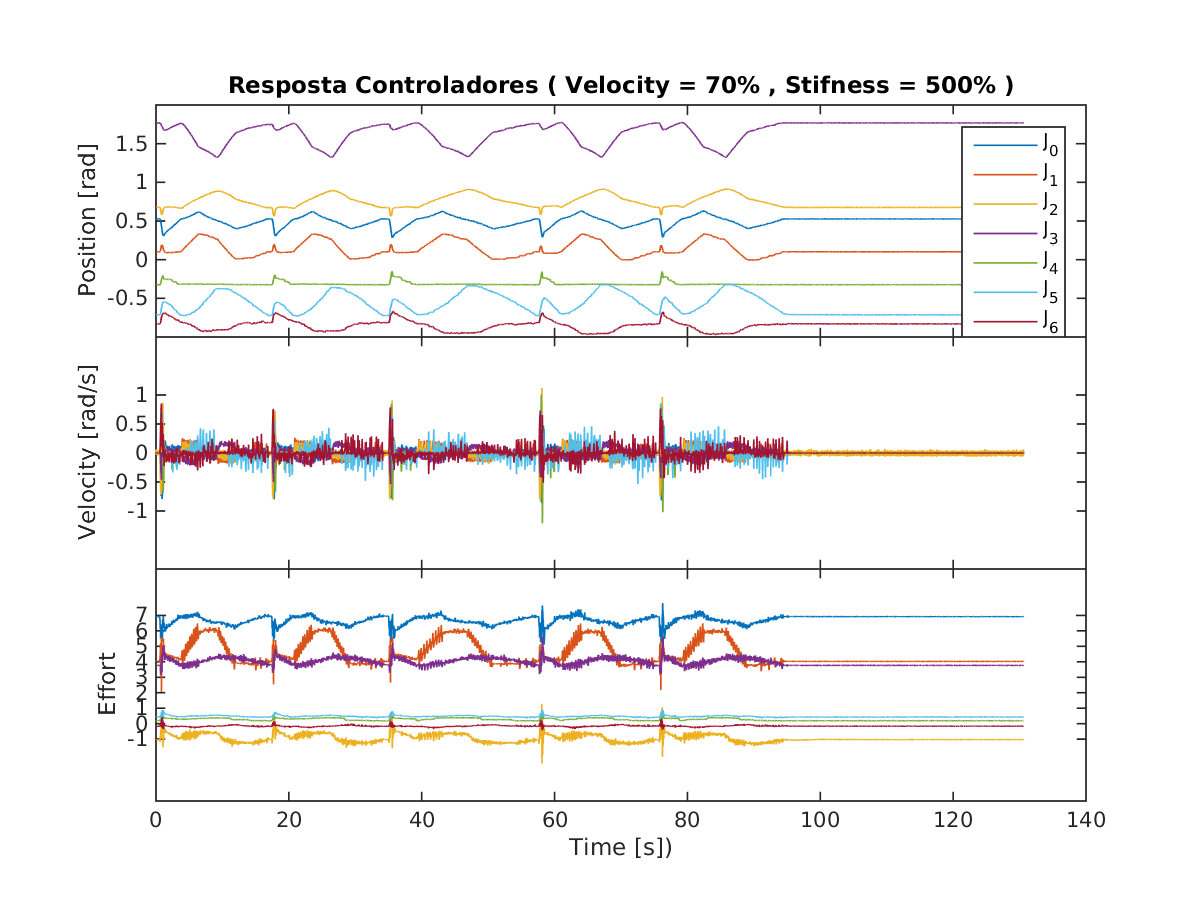
\includegraphics[width=0.8\linewidth,trim={2cm 1cm 2cm 0.5cm}]{tex/figs/squareStifff4stateEvalv70s500.png}
    \caption{Resposta dos Controladores de Juntas para Velocidade em $70\%$ e Stifness = $5$ }
    \label{fig:squareStiffMarcos}
\end{figure}

Apenas analisando a figura \ref{fig:squareStiffMarcos} podemos perceber alguns saltos a cada $18s$ na posição e na velocidades das juntas. Cada salto denota a transição entre um controlador e outro em decorrência do movimento de retorno a posição inicial. No que pode ser observado que cada controlador leva um tempo diferente para cumprir a trajetória, porém a resposta de todos é bem similar no formato da trajetória. Embora contenha toda a movimentação, este gráfico permite apenas uma visão geral do comportamento. Assim, a partir destes dados, foram extraídos os dados de cada junta como forma de detalhar a contribuição individual para o erro avaliado e o desenvolvimento da trajetória.

Os gráficos de cada junta são apresentados nas figuras \ref{fig:squareStiffJ9stateEval_J0v100s70} a \ref{fig:squareStiffJ9stateEval_J6v100s70}. Para todas é notado um salto no valor da referência. No entanto, ao observar a resposta de cada junta temos uma atenuação da variação rápida gerada pela transição entre um controlador e outro. Isto se deve a comportamento complacente do atuador série elástico que atua como um filtro passa baixa. A energia introduzida pela variação brusca é absorvida pela elasticidade do atuador e devolvida gradualmente ao sistema como observado mais claramente pelo gráfico de esforço de cada junta em que o salto na referência de posição é acompanhado de imediato por um salto no torque e por uma decida um pouco mais suave na curva da resposta do sensor. 

Dentre todas as juntas, a do ombro $J0$ apresentou o menor erro em relação a referência de controle, além de manter um torque aproximadamente constante ao longo de toda trajetória, figura \ref{fig:squareStiffJ9stateEval_J0v100s70}. Algo experado por ser a junta mais com o motor mais rápido e a maior rigidez.

\vspace{1cm}

\begin{figure}[H]
    \centering
    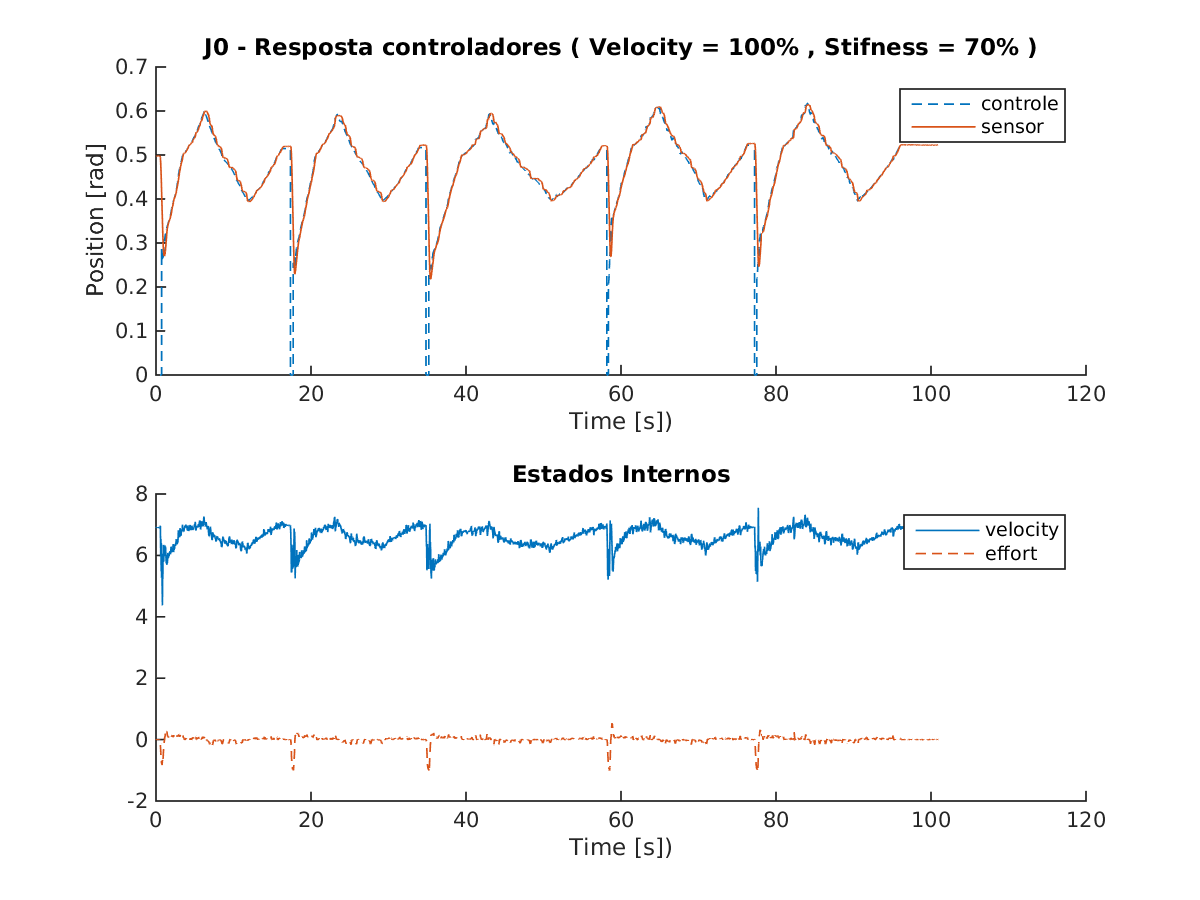
\includegraphics[width=0.6\linewidth,trim={2cm 1cm 2cm 2cm}]{tex/figs/squareStiffJ9stateEval_J0v100s70.png}
    \caption{Resposta Juntas $J0$ para Velocidade em $70\%$ e Stifness = $100\%$ }
    \label{fig:squareStiffJ9stateEval_J0v100s70}
\end{figure}

Para as demais juntas do ombro $J1$ e $J2$ o erro também foi pequeno e o torque foi aproximadamente constante. Sofrendo um pouco mais de variação em relação a $J0$ mas ainda dentro de uma margem pequena, como mostrado pelas figura \ref{fig:squareStiffJ9stateEval_J1v100s70} e \ref{fig:squareStiffJ9stateEval_J2v100s70}.

\vspace{1cm}
\begin{figure}[H]
    \centering
    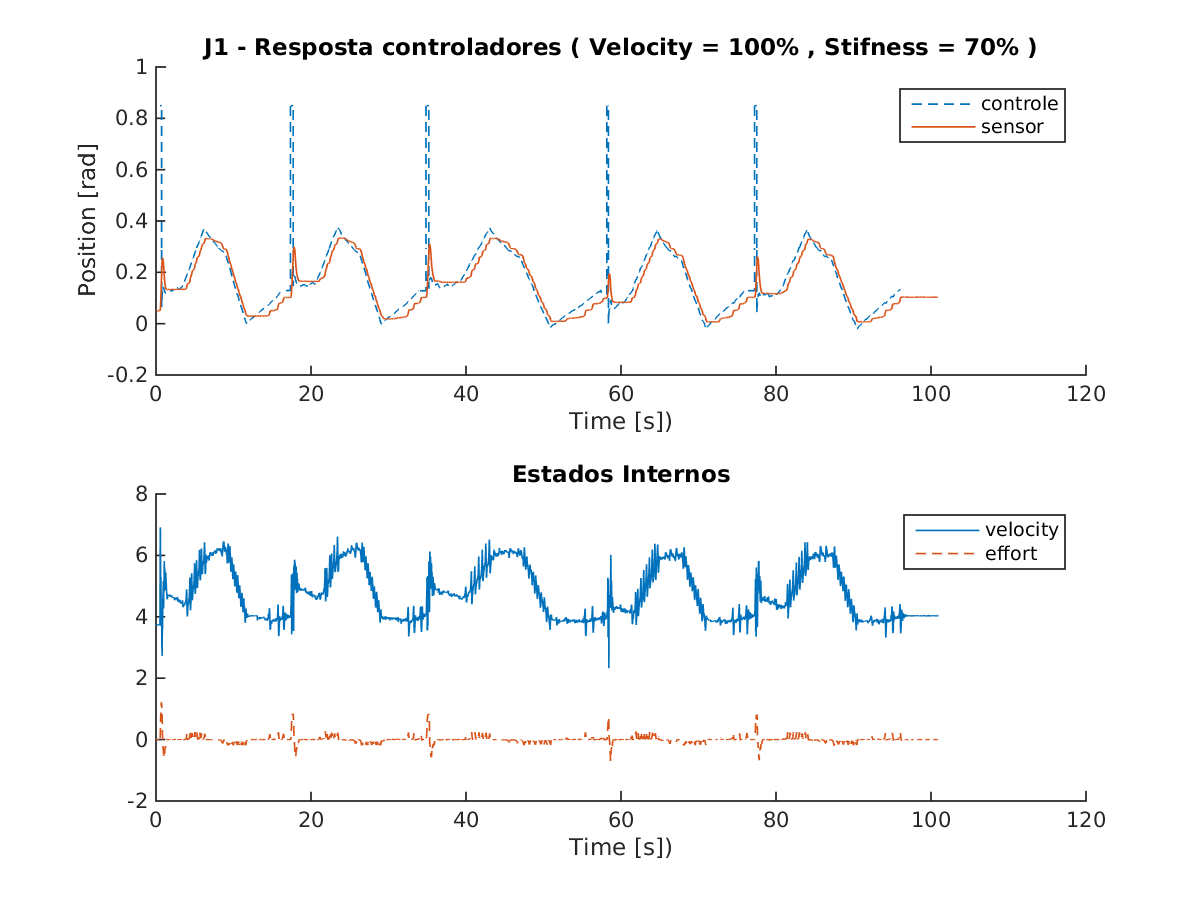
\includegraphics[width=0.6\linewidth,trim={2cm 1cm 2cm 2cm}]{tex/figs/squareStiffJ9stateEval_J1v100s70.png}
    \caption{Resposta Juntas $J1$ para Velocidade em $70\%$ e Stifness = $100\%$ }
    \label{fig:squareStiffJ9stateEval_J1v100s70}
\end{figure}

\vspace{1cm}

\begin{figure}[H]
    \centering
    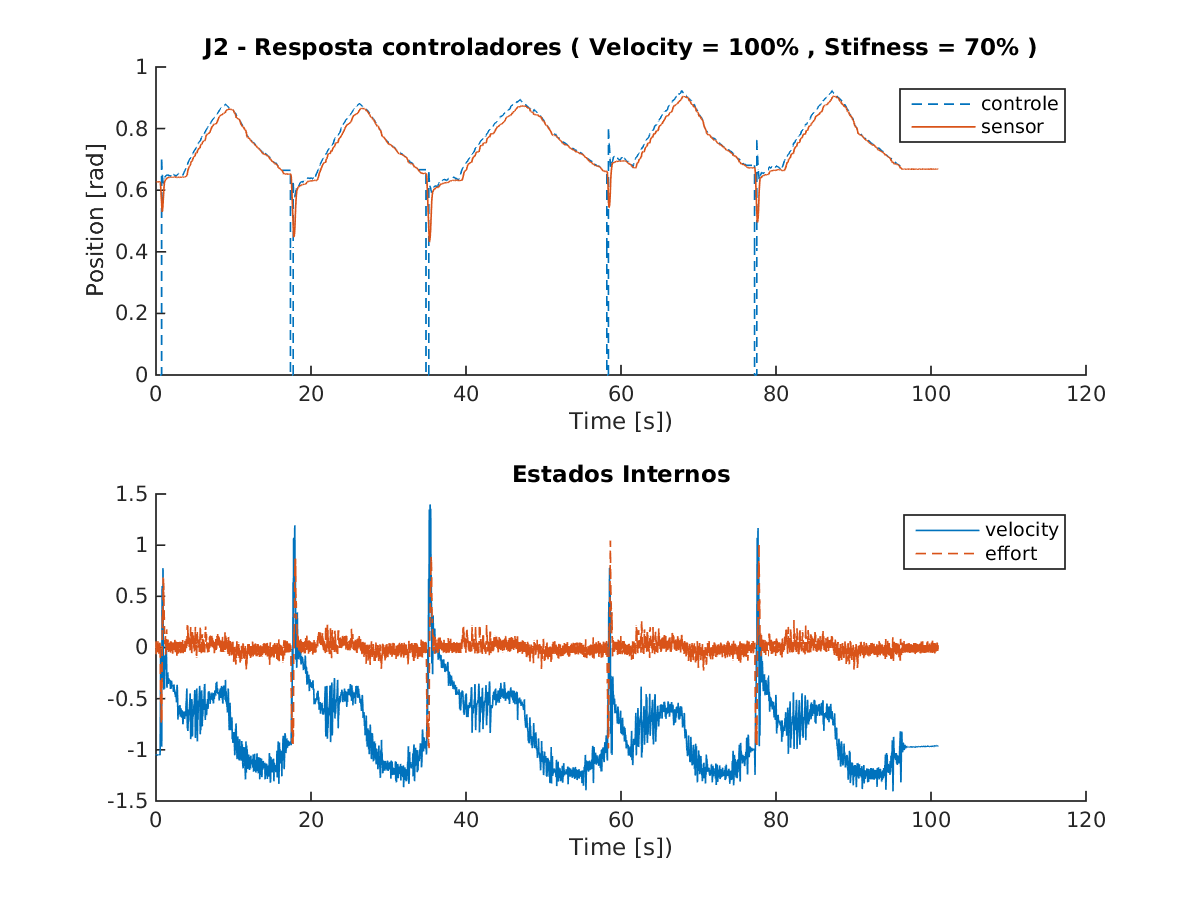
\includegraphics[width=0.6\linewidth,trim={2cm 1cm 2cm 2cm}]{tex/figs/squareStiffJ9stateEval_J2v100s70.png}
    \caption{Resposta Juntas $J2$ para Velocidade em $70\%$ e Stifness = $100\%$ }
    \label{fig:squareStiffJ9stateEval_J2v100s70}
\end{figure}

A junta $J4$ é a mais lenta dentre todas as juntas. A partir da figura \ref{fig:squareStiffJ9stateEval_J4v100s70}, nota-se uma resposta bem diferente em relação as demais. A junta não consegue acompanhar da mesma forma a referência e leva a uma acumulo de erro. Observa-se que velocidade sofre saltos próximos de $0.2 rad/s$ e o torque oscila bastante em determinadas regiões. Indicando que o controle esta trabalhando em regiões além da região linear de resposta da junta.

\vspace{1cm}

\begin{figure}[H]
    \centering
    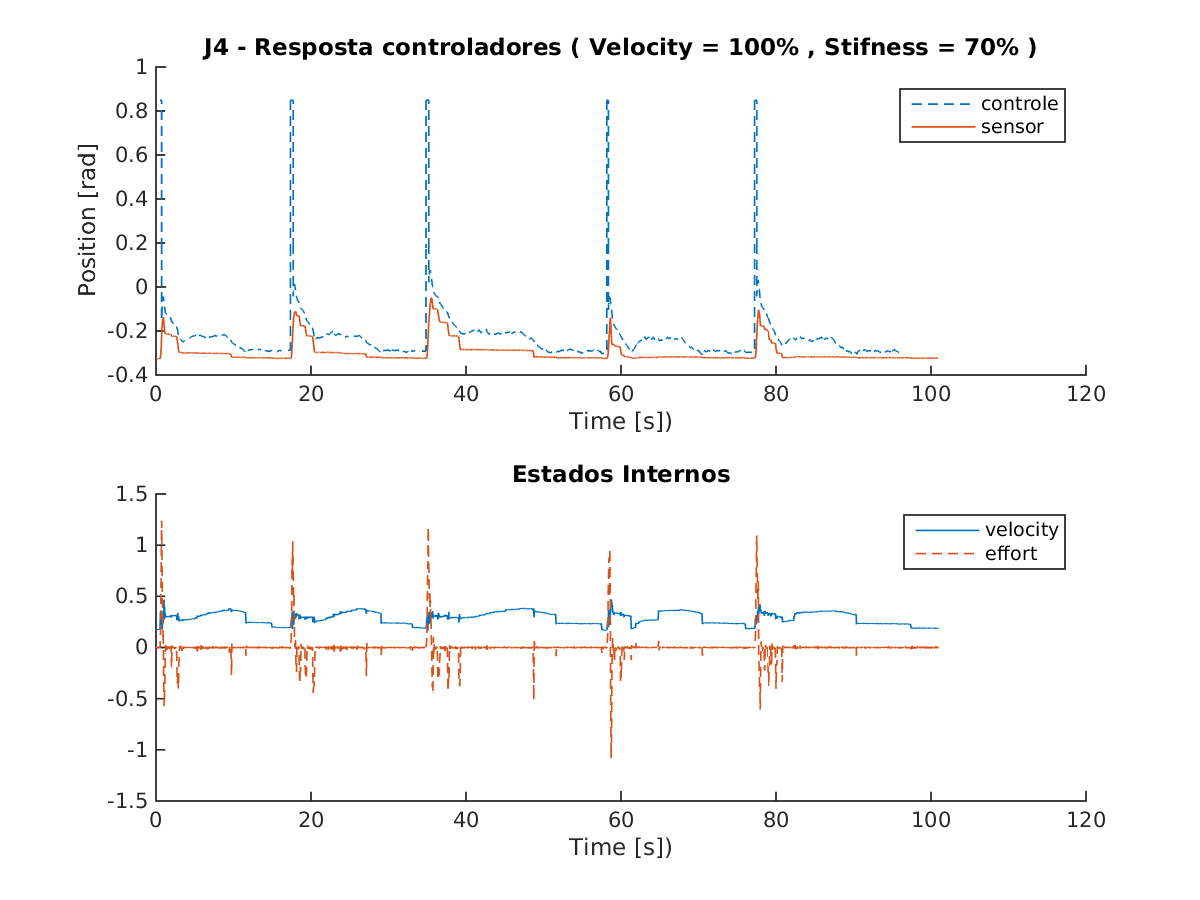
\includegraphics[width=0.6\linewidth,trim={2cm 1cm 2cm 2cm}]{tex/figs/squareStiffJ9stateEval_J4v100s70.png}
    \caption{Resposta Juntas $J4$ para Velocidade em $70\%$ e Stifness = $100\%$ }
    \label{fig:squareStiffJ9stateEval_J4v100s70}
\end{figure}

As juntas do pulso $J5$ e $J6$ estão acopladas mecanicamente pelo mecanismo de diferencial e separadas em $Yall$ e $Pitch$ através de um controlador dentro do PC. Em ambas é percebido o maior erro no acompanhamento da referência, similar ao ocorrido no experimento de resposta a degrau na figura\ref{fig:jointIdentification_exp3v70v100}. Porém é notado uma alta variação no torque da exercido pela junta nas figura \ref{fig:squareStiffJ9stateEval_J5v100s70} e \ref{fig:squareStiffJ9stateEval_J6v100s70}.

\vspace{1cm}

\begin{figure}[H]
    \centering
    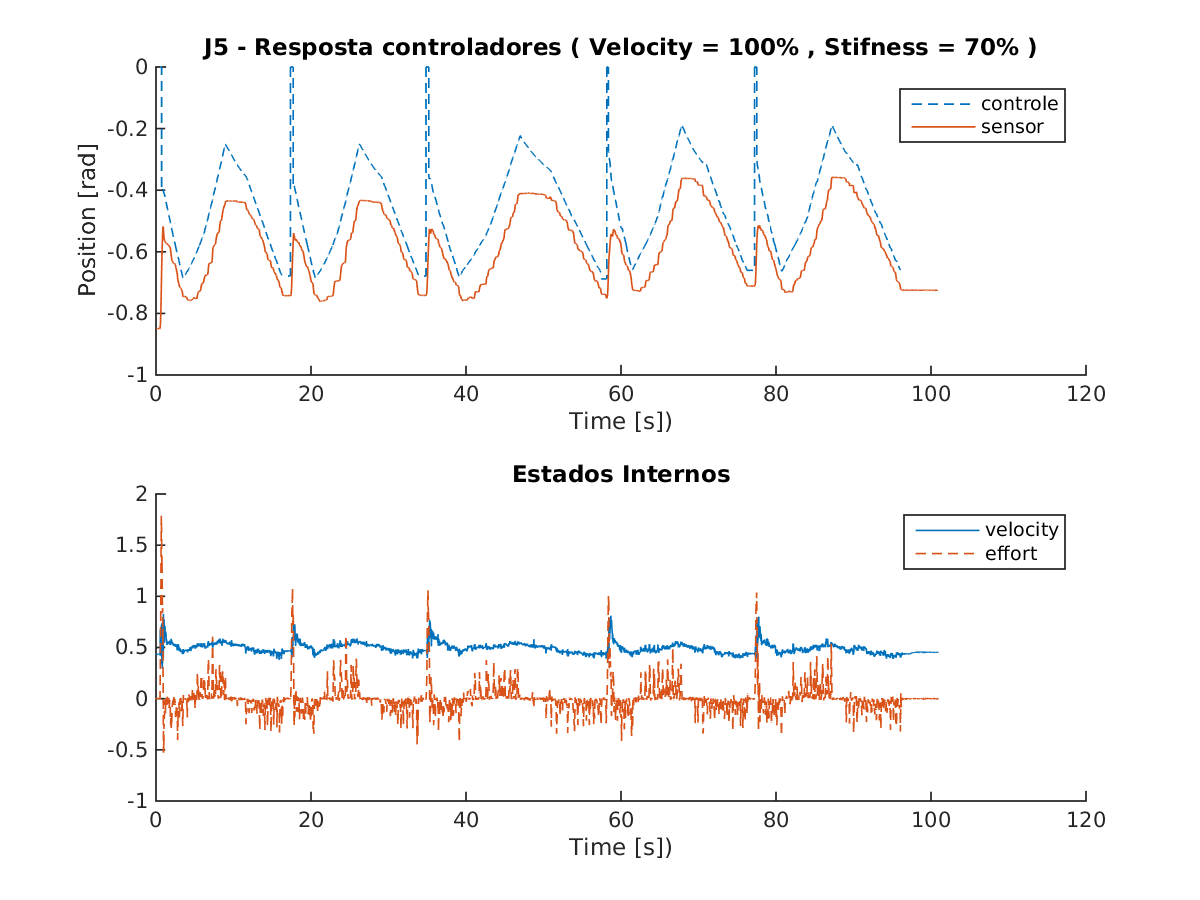
\includegraphics[width=0.6\linewidth,trim={2cm 1cm 2cm 2cm}]{tex/figs/squareStiffJ9stateEval_J5v100s70.png}
    \caption{Resposta Juntas $J5$ para Velocidade em $70\%$ e Stifness = $100\%$ }
    \label{fig:squareStiffJ9stateEval_J5v100s70}
\end{figure}

\vspace{1cm}

\begin{figure}[H]
    \centering
    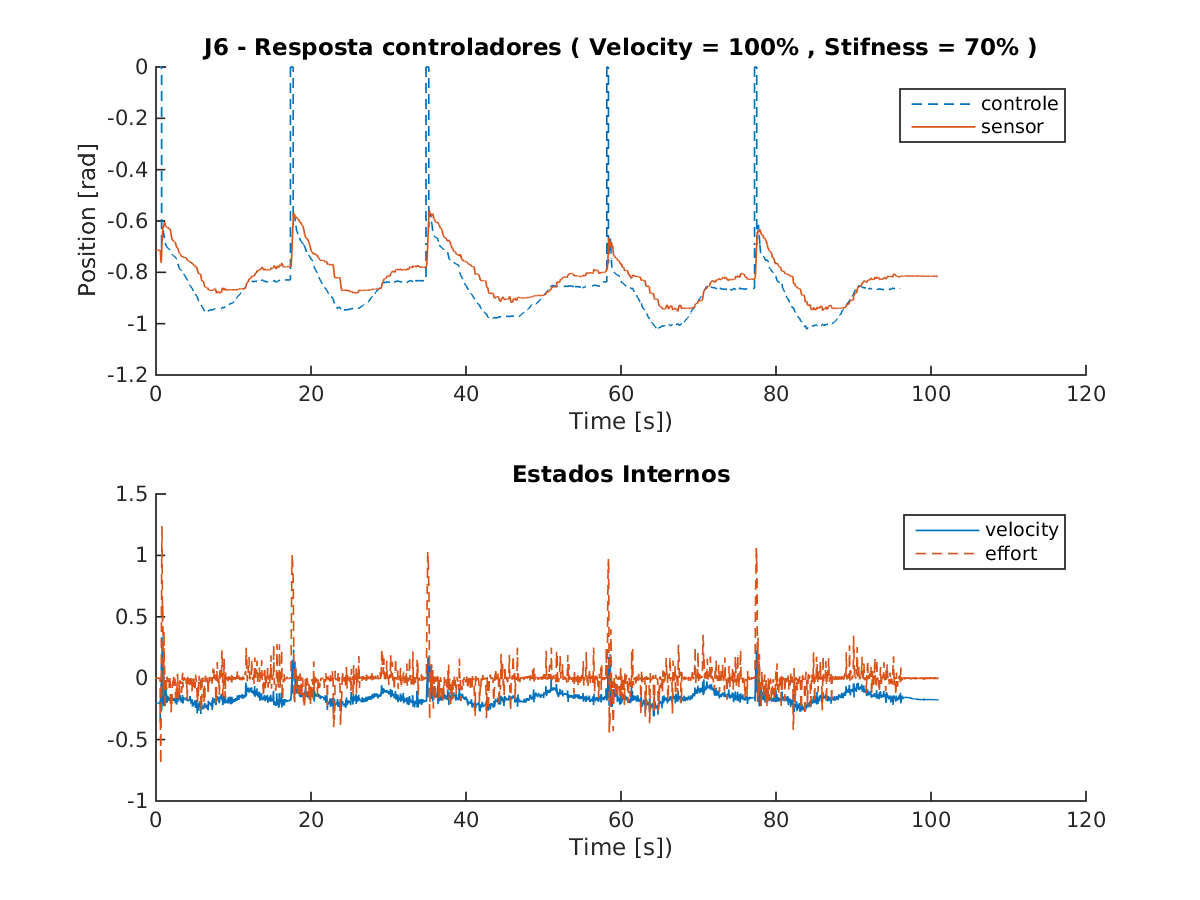
\includegraphics[width=0.6\linewidth,trim={2cm 1cm 2cm 2cm}]{tex/figs/squareStiffJ9stateEval_J6v100s70.png}
    \caption{Resposta Juntas $J6$ para Velocidade em $70\%$ e Stifness = $100\%$ }
    \label{fig:squareStiffJ9stateEval_J6v100s70}
\end{figure}

Naturalmente são as juntas mais próximo do efetuador e portanto toda a oscilação produzida pelas demais juntas é transmitida diretamente ao pulso. No entanto, tendo uma rigidez mais baixa, um erro grande em regime permanente acaba tendo um impacto grande no erro da orientação do efetuador. Já que dado a geometria do robô a orientação da posição de referência do efetuador está ligada diretamente a posição das juntas do pulso. Se considerar ainda que o ponto de referência usado está deslocado em relação ao centro do pulso diferencial, este erro de orientação será ainda refletido também em um erro de posição. Ao que concluímos que a maior contribuição para o erro da posição ocorre nas juntas associadas ao movimento do pulso.

% \begin{table}[H]
%     \centering
%     \caption{Avaliação torque por junta}
%     $$\begin{array}{cc|ccccccc}
%          \hline
%          V & S & J_0 & J_1 & J_2 & J_3 & J_4 & J_5 & J_6\\
%          \hline
%          1.00 & 0.90 & 2.6061 & 3.9737 & 1.9986 & 2.9634 & 0.44615 & 1.3359 & 1.3625\\
1.00 & 0.80 & 4.1501 & 3.7957 & 2.1348 & 2.7368 & 0.63212 & 1.0438 & 1.105\\
1.00 & 0.70 & 2.3535 & 3.7261 & 1.7106 & 2.0638 & 0.4362 & 0.92678 & 0.94839\\
1.00 & 0.50 & 2.3401 & 3.9314 & 1.4722 & 1.8769 & 0.41536 & 1.0929 & 0.9881\\
1.00 & 0.20 & 2.3457 & 2.9149 & 1.0301 & 1.5902 & 0.38187 & 0.61833 & 0.57759\\
0.70 & 5.00 & 2.9491 & 4.0569 & 2.3652 & 6.4136 & 0.64046 & 2.613 & 2.6923\\

%          \hline
%     \end{array}$$
%     \label{tab:squareStiff_jointEffort}
% \end{table}

% \begin{table}[H]
%     \centering
%     \caption{Esforço de controle por junta a partir da posição}
%     $$\begin{array}{cc|ccccccc}
%          \hline
%          V & S & J_0 & J_1 & J_2 & J_3 & J_4 & J_5 & J_6\\
%          \hline
%          1.00 & 0.90 & 0.040153 & 0.038567 & 0.032152 & 0.048204 & 0.043179 & 0.045582 & 0.039519\\
1.00 & 0.80 & 0.049253 & 0.029412 & 0.031939 & 0.046974 & 0.059088 & 0.059512 & 0.049572\\
1.00 & 0.70 & 0.038172 & 0.036375 & 0.035099 & 0.028686 & 0.035327 & 0.044673 & 0.036756\\
1.00 & 0.50 & 0.04301 & 0.039182 & 0.036592 & 0.048036 & 0.043263 & 0.042057 & 0.035923\\
1.00 & 0.20 & 0.037593 & 0.023241 & 0.037907 & 0.034623 & 0.013048 & 0.02187 & 0.017025\\
0.70 & 5.00 & 0.038125 & 0.031918 & 0.02218 & 0.056704 & 0.038798 & 0.049131 & 0.043834\\

%          \hline
%     \end{array}$$
%     \label{tab:squareStiff_jointControlEffort}
% \end{table}

\subsection{Controle de Rigidez}

O mesmo experimento foi feito para vários valores de rigidez. Nas figuras \ref{fig:squareStiffJ10stateEval_J6v100s90}, \ref{fig:squareStiffJ6stateEval_J6v100s50} e \ref{fig:squareStiffJ7stateEval_J6v100s20} são apresentados a resposta da junta $J6$ do pulso, para rigidez igual a $90\%$, $50\%$ e $20\%$ respectivamente. Os experimentos foram feitos para todo as juntas no entanto esta foi a que apresentou a maior variação. Onde foi observado que conforme a rigidez é reduzida o erro aumenta em relação ao controle. Com $20\%$ de rigidez o atuador varia pouco a posição e o maior dentre os 3 casos.

\vspace{1cm}

\begin{figure}[H]
    \centering
    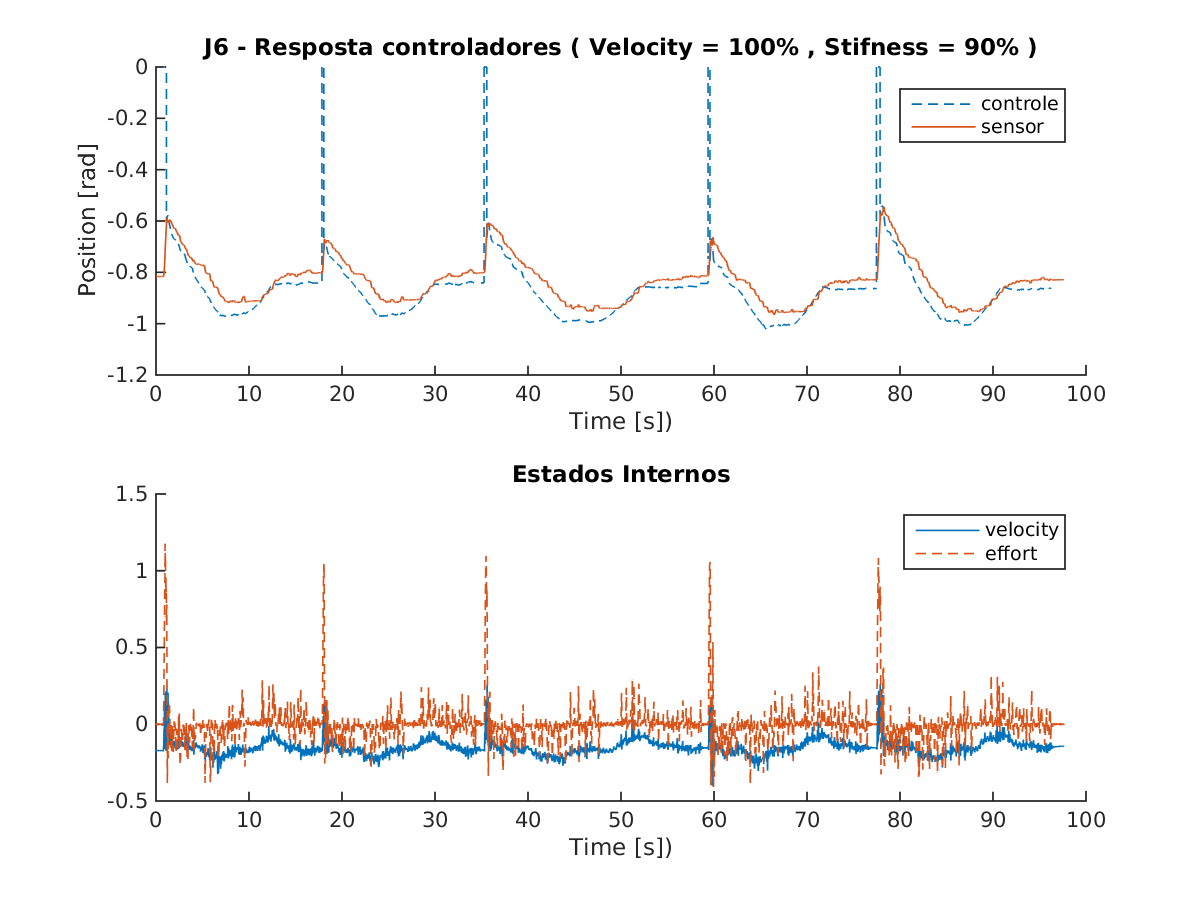
\includegraphics[width=0.6\linewidth,trim={2cm 1cm 2cm 2cm}]{tex/figs/squareStiffJ10stateEval_J6v100s90.png}
    \caption{Resposta Juntas $J6$ para Velocidade em $100\%$ e Stifness = $90\%$ }
    \label{fig:squareStiffJ10stateEval_J6v100s90}
\end{figure}

\vspace{1cm}

\begin{figure}[H]
    \centering
    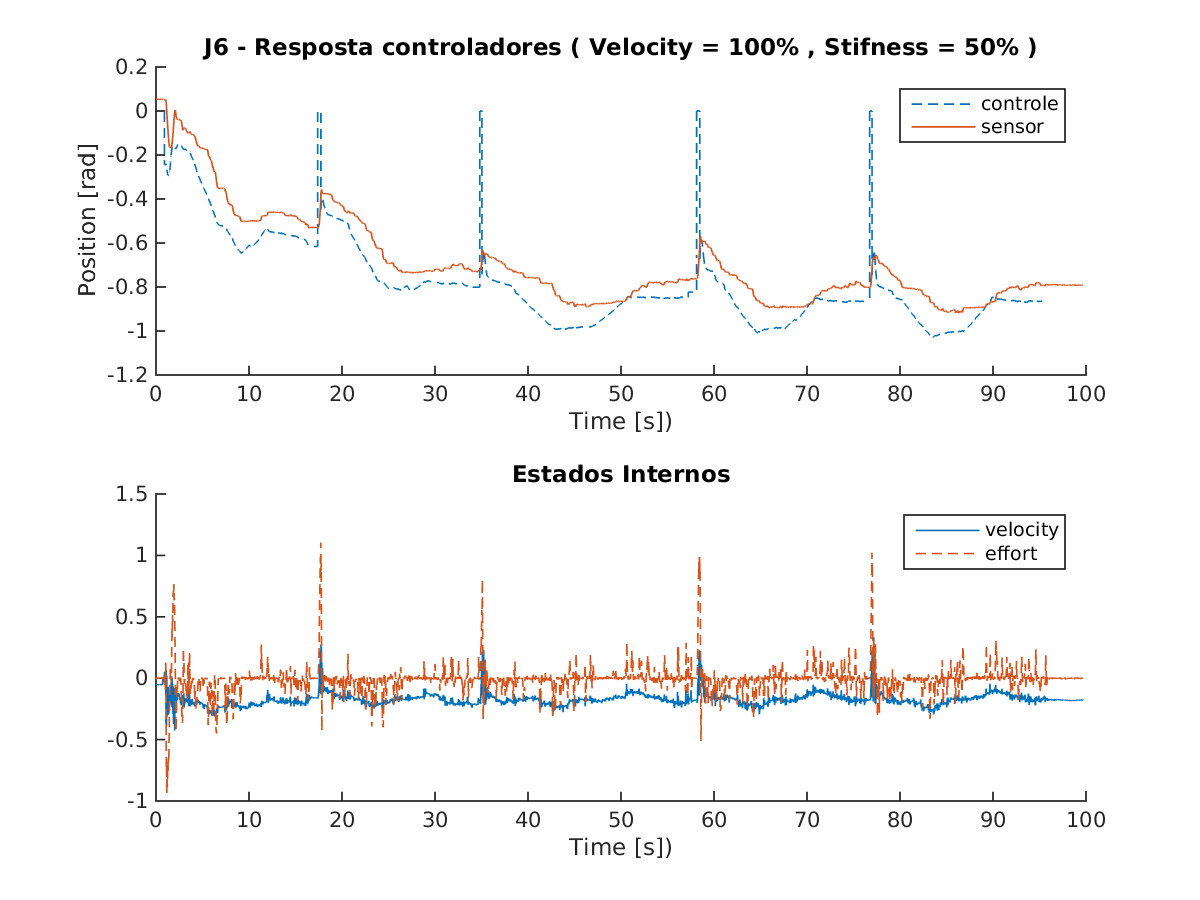
\includegraphics[width=0.6\linewidth,trim={2cm 1cm 2cm 2cm}]{tex/figs/squareStiffJ6stateEval_J6v100s50.png}
    \caption{Resposta Juntas $J6$ para Velocidade em $100\%$ e Stifness = $50\%$ }
    \label{fig:squareStiffJ6stateEval_J6v100s50}
\end{figure}

\vspace{1cm}

\begin{figure}[H]
    \centering
    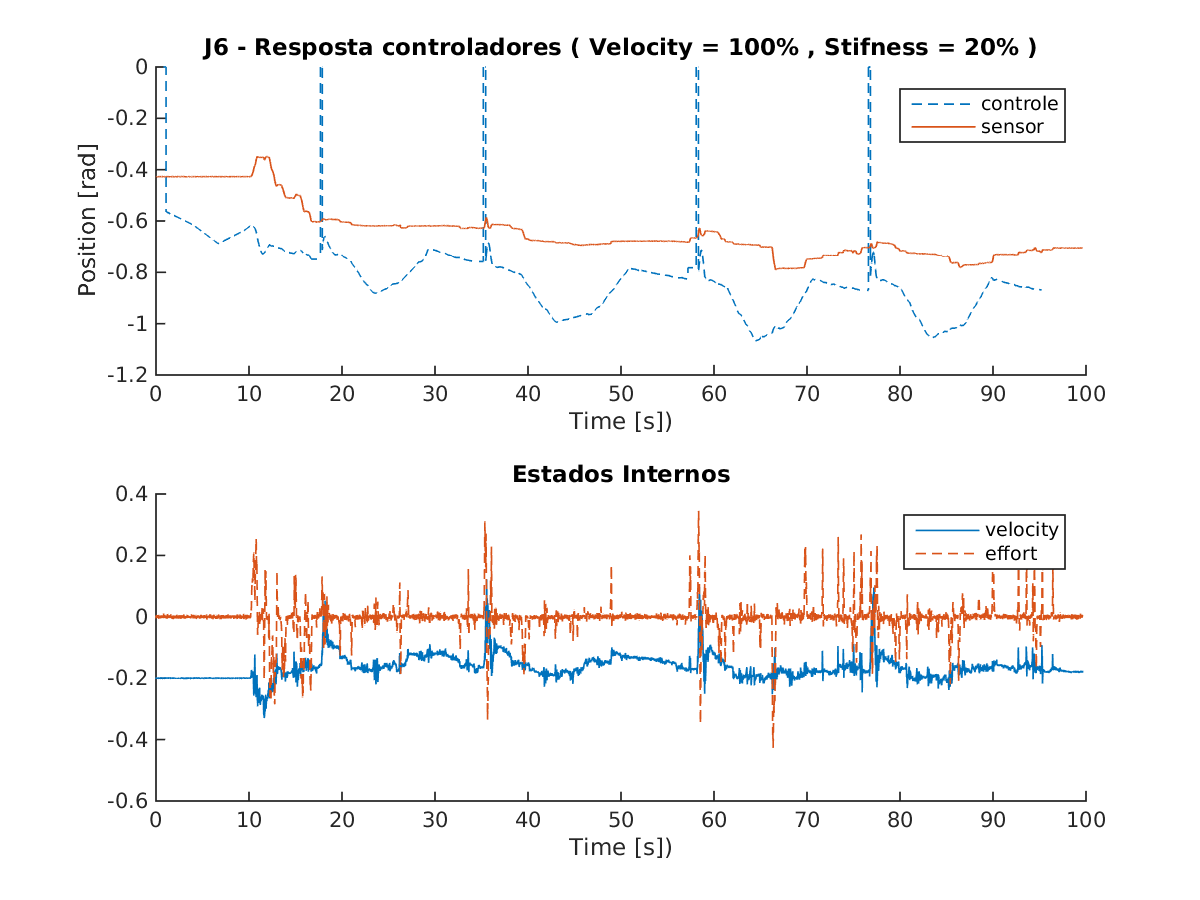
\includegraphics[width=0.6\linewidth,trim={2cm 1cm 2cm 2cm}]{tex/figs/squareStiffJ7stateEval_J6v100s20.png}
    \caption{Resposta Juntas $J6$ para Velocidade em $100\%$ e Stifness = $20\%$ }
    \label{fig:squareStiffJ7stateEval_J6v100s20}
\end{figure}

\section{Conclusão}

Juntando todas as análise foi percebido que o erro do pulso está tendo um peso significativo nos resultados obtidos para o erro. Pois como comentado, devido a geometria do braço, o pulso têm um papel significativo na rotação. E este efeito gera também a translação do ponto de referência do efetuador. O que mostra que a rotação está tendo um impacto significativo no movimento do braço que até então era inexplicado.

Observa-se também uma proporção inadequada entre a unidade de erro de posição e de orientação. Como a referência dos controladores é passada através de Quaternions Duais Unitários, a posição e a orientação estão sempre acompladas. Ainda que durante toda a trajetória a orientação de referência seja mantida, esta não é livre e compete com a tarefa de acompanhar a referência de posição da trajetória.

Como a descrição dos parâmetros do robô têm a distância sendo a avaliada em metros enquanto a orientação é medida sem radianos, esta proporção acaba influênciando na resposta do controlador. Embora seja unidades as unidades padrão, a proporção entre as unidades influência dinâmica do erro. Tal pode ser explicada da seguinte forma: Resgatando da definição de Quatérnions Duais Unitários, temos que os primeiros 4 elementos estão relacionados com a orientação e como se trata de um Quatérnion Unitário, cada deve variar entre $-1$ e $1$. De modo que a variação de 2 grau é gera um coeficiente $sen(\theta_x/2)$ =  $sen(2/2)$ = $sen(1)$ que é aproximadamente $pi/180$ = $0.017$. Como os parâmetros do robôs são representados em metros, podemos avaliar o coeficiente gerado pelo deslocamento de $2cm$ com $t_x/2$ = $0.02/2$ = $0.01$. Dado que o cálculo do erro definido pelos controladores em \cite{marcosps2016} trata todos os coeficientes do quatérnion dual com o mesmo peso, temos que o desvio de $2 graus$ gera um impacto maior que o desvio de $2cm$. O que é um pouco desproporcional se considerarmos que o lado do quadrado efetuado pela trajetória é de $10cm$ e foco da avaliação era a resposta da translação.

% Fundamentação
% - Qualidade do HW
O Meka foi implementado com componentes de alto desempenho seguindo a filosofia do mercado na sua época de lançamento. Embora hoje, outras tecnologias estão sendo incorporadas ao projeto de robôs complacentes como o uso de sistemas freios, esta plataforma ainda representa uma ótima plataforma para o estudo de controladores dinâmicos bem como cada uma dos componentes envolvidos. Como exemplo, o uso de atuadores série elásticos, embora estejam implementados no Meka com motores e sistemas de transmissão de ponta, podem também ser incorporados em outros projetos como solução aos problemas de instabilidade do controle na interação com superfícies rígidas em aplicações para locomoção. Ou ainda em aplicação de forças na área de fisioterapia.

% Desenvolvimento
No que tange ao sistema de controle implementado, foi percebido que nos trabalhos anteriores foi alcançado o limite de desempenho dos controladores de baixo nível implementado no sistema M3. No entanto, dado que o sistema de controle é completamente open-source e possui um sistema embarcado capaz de uma desempenho maior ainda existe um enorme potencial que pode ser explorado para uso em trabalhos futuros. Uma vez que as soluções implementadas incorporam técnicas de filtragem e controle dinâmico que podem ser aprimoradas.

% Resultados
% - Juntas
Os controladores de posição de juntas foram ajustados para responderem de forma similar para todas as juntas. Embora esta seja uma estratégia que permite que a resposta controle seja similar e facilite a avaliação dos controladores cinemáticos, na prática o comportamento o comportamento de cada junta é bem diferente. Para um ganho de desempenho, pode ser explorado a possibilidade de controladores ajustados para respostas diferente para cada uma das juntas. Em conjunto com as características particulares da geometria do braço, um desempenho melhor pode ser atingido, por permitir as juntas do ombro operarem com uma resposta mais rápida.

A técnica atualmente implementada para compensação da gravidade usa apenas a posição das juntas para uma gerar um torque em feedforward a partir do modelo cinemático e dinâmico do robô. Outras técnicas podem ser utilizadas para que as velocidade final e o torque possam também ajustadas. Também foi notado que o acoplamento entre a posição e a orientação introduzido por quatérnions duais pode ser explorado a partir das características das juntas do robô, uma vez que a composição do ombro e do pulso podem atuar como dois guibal em oposição permitindo um estudo maior da dinâmica da rotação no movimento do efetuador.

